\documentclass[a4paper,11pt]{article}
%\usepackage[pdftex]{graphicx}
\usepackage{amsmath}
%\usepackage[latin1]{inputenc}
%\usepackage{hyperref}
%\usepackage[T1]{fontenc}
%\usepackage[utf8]{inputenc}
%%GD Quand je mets usepackage[utf8]{inputenc} je n'arrive plus à compiler la biblio
%J'ai essayé de débuger : je n'y suis pas arrivé
\usepackage{rotating}
\usepackage{setspace}
\usepackage{lscape}
\usepackage[round]{natbib}
\usepackage{multirow}
\usepackage{rotating}
\usepackage{vmargin}
\usepackage{epstopdf}
\usepackage{hyperref}
\usepackage{float}
\usepackage{caption}
\usepackage[tableposition=top]{caption}
\usepackage{ bbold }
\usepackage{ upgreek }
\usepackage{comment}
\includecomment{commentGD}
\usepackage[draft]{todonotes}
%\usepackage[disable]{todonotes}
%%GDPour cacher les notes, \usepackage[disable]{todonotes}


%\usepackage[nolists, figuresfirst]{endfloat}
%\usepackage{sidefloat}

\setlength{\abovecaptionskip}{-8pt}

%\usepackage[usenames]{color}
%\definecolor{grey}{rgb}{0.35,0.35,0.35}
%\definecolor{webdarkblue}{rgb}{0,0,0.4}
%\definecolor{orange}{rgb}{0.7,0.2,0.05}


%\usepackage[pdfcreator={PDFLaTeX}, pdfproducer={PDFLaTeX}, pdfstartview=FitH, pdfpagemode=UseOutlines, pagebackref=false, colorlinks={true},
%citecolor={webdarkblue}, linkcolor={webdarkblue},
%urlcolor={webdarkblue}]{hyperref}



%\addtolength{\oddsidemargin}{-0.4in}
%\addtolength{\evensidemargin}{-0.4in}
%\addtolength{\textwidth}{0.8in} \addtolength{\topmargin}{-0.85in}
%\addtolength{\textheight}{1.7in}
\renewcommand{\baselinestretch}{1.2}





\setmarginsrb{3cm}{2cm}{3cm}{2cm}{0,5cm}{0,5cm}{0,3cm}{0,5cm}



% commands

\newcommand{\bi}{\begin{itemize}}
\newcommand{\ei}{\end{itemize}}
\newcommand{\be}{\begin{enumerate}}
\newcommand{\ee}{\end{enumerate}}
\newcommand{\bd}{\begin{description}}
\newcommand{\ed}{\end{description}}
\newcommand{\beqa}{\begin{eqnarray}}
\newcommand{\eeqa}{\end{eqnarray}}
\newcommand{\beq}{\begin{equation}}
\newcommand{\eeq}{\end{equation}}
\newcommand{\bs}{\bigskip}
\newcommand{\A}{$^a$}
\newcommand{\B}{$^b$}
\newcommand{\C}{$^c$}

\begin{document}



\title{\textsc{Beyond the Iceberg Hypothesis: \\Opening the Black Box of Transport Costs}} %\thanks{We are especially grateful to XXX. Part of this research was funded by the French Agence Nationale de la Recherche (ANR), under grant ANR-11-JSH1 002 01. Finally, any remaining errors are ours.}}}
%We also thank participants at the EEA 27\textsuperscript{th} Congress (Oslo), ETSG 13\textsuperscript{th} meetings (Copenhagen), INFER Workshop (Orleans), 45\textsuperscript{th} Congress of the Canadian Economic Association (Ottawa), IAW Workshop (Tubingen), and seminars at WTO, Strathclyde University, OFCE and EQUIPPE-University of Lille.
\author{Guillaume \textsc{Daudin}\thanks{%
Universit\'{e} Paris-Dauphine, PSL Research University, LEDa-DIAL, UMR 225, France \&
SciencesPo, Observatoire Français des Conjonctures \'{E}conomiques (OFCE), France}  \qquad J\'{e}r\^{o}me \textsc{H\'{e}ricourt} \thanks{Universit\'{e} de Lille - LEM-CNRS UMR 9221, France \& CEPII, France}\qquad Lise \textsc{Patureau}\thanks{Universit\'{e} Paris-Dauphine, PSL Research University, LEDa, France } }


\date{July 2017}
 \maketitle
\bigskip

\begin{abstract}
Following \cite{samuelson1954}, standard models of international trade have usually relied on modelling trade costs as an ad-valorem tax equivalent. However, many common empirical facts suggest the existence of additive costs. This paper provides new empirical results that support this view. To do so, we exploit information contained in the US imports flows database over 1974-2013, distinguishing by transport mode (air and ocean). Two main results emerge. First, we show the additive component of transport costs is sizeable, with mean values over the period of 1.8\% and 2.9\% of the export price in air and maritime transport respectively. Further, taking additive costs into account significantly improves the fit of the modelling of transport costs. Second, we show the importance of integrating the additive component in accounting for the time trend of international transport costs. We thus show that the decrease of international transport costs observed in the data is mostly attributable to a reduction in the \textit{pure} transport costs rather than to trade pattern composition effects. These results therefore confirm the importance of the additive component in accounting for international transport costs.

\end{abstract}

\thispagestyle{empty} \pagestyle{plain} \setcounter{page}{1}



{\normalsize JEL classification: F14, N70, R40\newline
Keywords: Transport costs estimates, transport costs determinants, non-linear econometrics, period 1974-2013, additive transport costs }

{\normalsize \vspace{0cm} }

{\normalsize \titlepage }

{\normalsize \newpage }

%\begin{spacing}{1.5}

\section{Introduction}



\noindent Trade costs are central in international economic analysis. In particular, they are considered a major obstacle to international economic integration and international trade flows. According to \cite{Jacks08}, the trade cost decline explains around 55\% of the pre-World War I trade boom and 33\% of the post-World War II trade boom, while the abrupt rise in trade costs explains the inter-war trade collapse. After 1950, average trade costs fell by 16\%, notably through the reduction of policy trade costs promoted through the GATT (WTO as off 1995) multilateral agreements.
Based on panel data, \citet{novy13} finds  that U.S. trade costs with major trading partners declined on average by about 40 percent between 1970 and 2000.
Yet, several papers (mostly based on empirical estimates of the gravity equation) have shown that trade costs still remain a major obstacle to trade (\citealp{Head_Mayer04} and \citealp{Disdier_Head08}). Using data over 1989-2000, \citet{anderson_wincoop_jel} thus estimate that average international trade costs for industrialized countries represent a 74\% markup over production costs.

Defined as the costs associated with the exchange of goods across national borders, trade costs are usually split into transaction costs (information costs, contract enforcement costs, costs associated with the use of different currencies...), policy costs (tariff  and non-tariff costs), time costs (time to ship goods) and transport costs \emph{per se}. In this vein, \citet{anderson_wincoop_jel} obtain that around 30\% of international trade costs are attributable to transport costs. Equivalently, international transportation costs would represent a 21\% markup over production costs. Further, the sizeable elasticity of trade with respect to freight costs obtained by \cite{Behar_Venables}, by around -3, suggests a non-negligible impact of transport costs on trade flows. If much of trade-policy barriers have been removed over the second half of the 20th century, these findings point out that the transport costs component of the overall trade costs remain large and deserve attention. This is accordingly the focus of the paper.\smallskip


Following \citet{samuelson1954}, standard models of international trade have usually modelled trade costs as an \emph{ad-valorem} tax equivalent (ie, as a constant percentage of the producer price per unit traded, part of the ``iceberg cost'' hypothesis)\footnote{Rigourously speaking, the ``iceberg cost'' includes both the ad-valorem dimension of trade cost and the fact that these costs are paid in terms of the good that is traded. As this last element is irrelevant in our case, we use the terms ``iceberg'' and ``ad-valorem'' interchangeably, as commonly made in the literature.} However, many common empirical facts support the existence of additive costs (i.e., cost per unit exported). As documented by \citet{Irrazabal_2015}, pricing structure in shipping, additive tariffs, distribution costs... often exhibit (at least partly) an additive structure. The structure (additive vs ad-valorem) of transport costs is far from being anecdotal, as the literature has long emphasized its role in shaping the pattern of trade flows. As pointed out by the seminal paper of \cite{alchian}, the relative price of two varieties of some good will depend on the level of trade costs as long as they display an additive component. In this context, the relative demand for more expensive/higher quality product goods increases with trade costs (``shipping the good apples out''). \citet{Lashkaripour-mimeo-2016} challenges this view. He finds supporting evidence for the \emph{ad-valorem} assumption by taking into account the fact that more expensive goods are systematically heavier and hence more costly to transport. One can yet be concerned by the generality of this result. By nature, his study is restricted to goods that are enumerated by items in the statistics (they represent 60\% of US imports). Furthermore, while the positive correlation between weight and price seems reasonable for goods from the second industrial revolution like cars, it is dubious in the case of ITC goods which importance has been rising since 1994 (the end point of Lashkaripour's study). Besides, a number of empirical papers provide a strong empirical support to the role of additive costs in international trade costs. Based on a firm-product-level database of French exporters, \citet{martin2012} finds that firms charge higher fas unit values on exports to more remote countries, in contradiction with the ad-valorem hypothesis. \citet{hummels_skiba} estimate the elasticity of freight rates with respect to price to be well below unity. Also, their estimates imply that doubling freight costs increases average fas export prices by 80-141 percent, consistent with high quality goods being sold in markets with high freight costs. These findings deliver strong empirical support in favor of the Alchian-Allen conjecture.
\smallskip


Beyond the positive aspect, several recent papers also point out the normative implications of additive trade costs. \citet{sorensen2014} extends \citet{melitz}'s seminal model of international trade by including additive trade costs, in addition to the ad-valorem component. A key analytical result is that the welfare gain from a reduction in trade barriers is higher for a decrease in additive costs than a decrease in ad-valorem costs.\footnote{This is due to the alteration of relative prices in a heterogeneous-firms trade framework. Lower additive trade costs reduce the export market prices of the highly performing exporters relative to lowly performing exporters and thus shift relative market shares among exporters towards the highly performing exporters - this of course does not happen with iceberg costs. Total export sales are then reallocated between a smaller number of high productivity firms. Therefore, the expected profits from exporting prior to entry increase all other things being equal by more in the case of lower per-unit costs, driving up incentives to enter the industry and bringing eventually the welfare enhancing intra-industry reallocations highlighted in \citet{melitz} framework.} Calibrating on Norwegian firm-level data for 2004, \citet{Irrazabal_2015} find that an additive import tariff reduces welfare and trade by more than an identically-sized ad-valorem tariff. While these results suggest that important welfare gains can be achieved by reducing additive trade costs, not much progress has been done in quantifying such gains. One potential reason is the lack of an empirical characterization of the additive component of trade costs.\footnote{The one exception being \citet{Irrazabal_2015}, upon which we come back later.} One objective of the paper is to fill this gap. \bigskip


Our paper provides an empirical decomposition of the structure of transport costs over time, by explicitly distinguishing between ad-valorem and additive parts. In this respect, the paper is related to the literature that challenges the dominant role of iceberg costs in international trade.\footnote{On top of the previously cited papers about additive costs, our paper also relates to \citet{Alessandria-et-al-AER-2010}, \citet{Hornok-et-al-RES-2015} or \citet{Hornok-et-al-JIE-2015}, which point out the role of per-shipment costs (among which, administrative costs) in generating some ``lumpiness'' in international trade transactions.}
We quantitatively assess the size and the importance of the additive component in international transport costs, that we measure as the difference between the import and the export prices, based on the US Imports flows over 1974-2013. Obviously, exploiting this database is not immune of limitations, in particular as it restricts our scope of study to the monetary dimension of international transport costs. Our measure being based on the gap between export and import prices, it necessarily omits the other dimension of transport costs related to the time value of goods in transit. According to \citet{anderson_wincoop_jel}, the 21\% markup over production costs coming from transport costs includes both directly measured freight costs (10.7\%) and 9\% tax equivalent of ``indirect'' costs related to the time value of goods on their way to their export market (including holding cost for the goods in transit, inventory cost due to buffering the variability of delivery dates, preparation costs associated with shipment size...). However, the evidence summarized in \citet{anderson_wincoop_jel} points to a persisting importance of direct transport costs, especially compared to other trade barriers: They remain more important than, e.g., policy barriers (8\% tax equivalent), language barrier (7\%) or information cost (6\%). \citet{Hummels_1999} mentions a bunch of papers which all point that transport costs pose a barrier similar in size, or larger than tariffs. In the same vein, \citet{limao_venables} highlight the importance of infrastructures for trade costs in general, through their impact on transport costs. Furthermore, our data is based on a single and reliable customs origin with a wide time and geographical coverage, and it allows us extracting a direct transport cost measure thereby limiting the measurement error bias. Therefore, we strongly believe exploiting this database may deliver useful and reliable insights on the structure of international trade costs.
Closely related to our paper is the work by \citet{Irrazabal_2015}, which develops a structural framework for inferring additive trade costs from firm-level trade data. Based on Norwegian exports in 2004, they find that additive trade costs are about 14\% of the median consumer price. If our study covers a narrower set of trade costs focused on transport costs, we reach a similar conclusion to them, that points out the important role of the additive component of international transport costs. Our work differentiates from them though, in two main aspects. First, our empirical analysis allows us to provide a quantitative measure of the levels of both the iceberg and the additive trade costs. Second, we exploit exhaustive information about the imports flows of the US over a large time span from 1974 to 2013. In this respect, our results deliver a broader view of the magnitude of additive costs in international trade over time.\smallskip


By exploiting the time coverage of our database, our paper also relates to a second strand of the international trade literature, that studies the patterns of trade costs over time, such as \cite{hummels2007} and \cite{Behar_Venables}. Many argue that transport costs have substantially decreased with technological advance in transportation, infrastructure development and new communication technologies (see \citealp{Lafourcade_Thisse}). \cite{Glaeser04} find that, over the twentieth century, the cost of moving goods have declined by over 90\% in real terms. However, \cite{hummels2007} points out the importance of the composition effects in the characterization of time trends of international transport costs. If we share this view with \cite{hummels2007}, we reach a different result though. In contrast to \cite{hummels2007},\footnote{Over 1974-2004, \cite{hummels2007} obtains a stronger decline in transportation costs when the composition effects by origin country and by product have been removed, in both air and ocean transports.} our results tend to downplay the role of trade composition effects in accounting for the decline of international transport costs observed since 1974. Importantly, this can be attributed to the role of the additive component, which modifies the decomposition of the trend reduction of transport costs between the one attributable to trade composition effects and the reduction in the ``pure'' transport costs. In both air and ocean transports, we thus find that this last dimension is the main driver of the reduction of international transport costs observed over time.


Our findings can be summarized in three main points.

First, our theoretically agnostic approach provides a fairly simple framework for measuring both ad-valorem and additive parts of transportation costs. We thus obtain that the mean values over 1974-2013 of iceberg costs are equal to 2.5\% and 3.2\% of the export price in air and ocean transport respectively, whereas the additive component amounts to 1.8\% and 2.9\%. To our best knowledge, our paper is the first to provide such an extensive quantitative measure of both ad-valorem and additive costs in total transport costs.\footnote{Given their database and their methodology, \citet{Irrazabal_2015} can only identify the ratio of the additive to the ad-valorem cost ($\frac{t_{ik}}{\tau_{ik}}$ in our terminology), that they interpret by expressing it in terms of the median export price by country-product ($\bar{\widetilde{p}}_{ik}$). By contrast, our estimation strategy enables us to uncover both values of the ad-valorem and the additive costs $\tau_{ik}$ and $t_{ik}$ separately, in terms of the country-product export price $\widetilde{p}_{ik}$.}  This represents a valuable insight for calibrating related international trade models.

Second, we provide an empirical assessment of what standard international trade models lose by skipping additive transport costs. Quantitatively, the omission of the additive term leads to overestimate the ad-valorem component by roughly a factor 2. On average over the whole period, biased estimate for ad-valorem is 5\% for air and 6\% for vessel, while unbiased estimate is respectively 2.5\% and 3.2\%. We also show that taking additive costs into account significantly improves the fit of the modelling of transport costs, through various measures of ``goodness-of-fit'', for both transport modes and years.

Third, we exploit the time dimension of our database to document the patterns of transport costs over time. Between 1974 and 2013, we thus find that transport costs have decreased by roughly 50\% in air shipping and 60\% in maritime shipping, and of same order of magnitude for both additive and iceberg components. Importantly, we find that most of this decline can be attributed to a reduction in the ``pure'' transport costs. Investigating this result further, we show that taking into account the additive component plays a key role in assessing the role of composition effects in the time trends of international transport costs. These results therefore confirm the importance of the additive component in accounting for international transport costs.\smallskip



The paper is built as follows. \ref{sec:data_method} presents our data and our  methodology. In Section \ref{sec:results_decomposition}, we provide results about the size and the role of the additive component of transport costs. After reporting the mean values over the period (by transport mode), we show how introducing additive transport costs improves the modelling of transport costs. Section \ref{sec:results_trends} characterizes the trends of transport costs (by transport mode) over the period 1974-2013. Section \ref{sec:robustness} provides some robustness checks of our results. Section \ref{sec:conclu} concludes.

\section{Data Sources and Empirical Methodology \label{sec:data_method}}

\textbf{integrer relecture Jerome sur cette section}

\subsection{A measure of Transportation Costs}

Our analysis of transportation costs consists in exploiting the difference between commodity-level export and import prices, as in \cite{hummels2007} (among others). The database we use to construct our measure of transport costs comes from US annual Imports of Merchandise provided by the Census bureau,\footnote{More information available at: \url{http://www.census.gov/foreign-trade/reference/products/catalog/fl_imp.txt}} spanning from 1974 to 2013. We first use customs values, quantities and freight costs to recover free-alongside (fas) and cost-insurance-fret (cif) prices, by goods, country of origin and transportation mode.\footnote{The related literature commonly refers to the fob price rather than the fas price. While both are closely related, we refer to the fas price as the price considered by the US Foreign Trade Statistics.} More precisely, the (unit) fas price is computed as the total ``customs value'' in the US trade statistics divided by the shipping weight; in other words, it is the price for one kg of the good net of transportation costs. The cif price is then computed as the sum of the customs value and freight charges, once again divided by the shipping weight. Our dependant variable is finally computed as the ratio of the cif price divided by the fas price. Higher than 1, the variable provides therefore with a measure of transport costs as a proportion of the good's price, an \emph{ad-valorem} equivalent. This is a quite standard and widespread strategy, as emphasized by \citet{anderson_wincoop_jel}.

It is worth acknowledging that using this dataset encounters some limitations. First, it restricts our analysis to the study of international transport costs, as our measure of the cif-fas price gap only covers freight, insurance and handling costs. It is thus silent about the others dimensions of international trade costs, unlike \citet{Irrazabal_2015}. Further, in terms of transport costs \textit{per se}, our measure based on the cif-fas price gap omits the other dimension of transport costs related to the time value of goods in transit. According to \citet{anderson_wincoop_jel}, the 21\% markup over production costs coming from transport costs includes both directly measured freight costs and 9\% tax equivalent of the time value of goods in transit. In this respect, it is true that using this dataset embraces a partial view of international transport barriers.

Yet, we believe that our analysis delivers valuable insights on this topic. Indeed, using this dataset has (at least) three main advantages. First, this dataset delivers a strong statistical reliability arising from a single, trustworthy, customs origin. Based on customs declarations, the US Imports database inventories all imports (both values and quantities) by country of origin to the United states at the HS 10-digit level, with a concordance code to the SITC 5-digit coding system. In addition, the database reports information regarding freight, insurance and handling expenditures by transportation mode (ocean (or ``vessel'') and air). The first will be crucial to compute transport costs (see below), the second will allow to enlighten substantial differences in the dynamics of transport costs across transportation mode. Second, using this dataset allows us to have the import price of the good, next to the export price. This is highly valuable, as we can estimate both the \textit{levels} of the iceberg costs and of the additive costs. This strongly differentiates us from \citet{Irrazabal_2015}, who can only estimate the ratio of additive costs as a share of the median total consumer price. Third, this dataset is available over a long time span. We are thus able to exploit information on a yearly basis from 1974 to 2013. \cite{hummels2007} preceded us in investigating the time dimension of this database. However, our paper differentiates from his work in two main respects. First, we extend the time coverage to the more recent period up to 2013, while \cite{hummels2007} stops in 2004. As we show in Section \ref{sec:results_trends}, covering the time period over the recent years delivers interesting insights regarding the trends in air shipping costs. Second, we study the time trends of transport costs by disentangling the additive from the iceberg components. This proves to be important in the characterization of transport costs changes over time, in particular in air shipping.\smallskip

We estimate international transport costs at the 3-digit classification level, even if data series on the cif and fas prices are available at the 5-digit classification level. As detailed below, the use of a nonlinear estimator triggers computational limitations that limit the level of possible detail, especially when covering a long period of time. Yet, we ensure the robustness of these results by conducting the estimations at the 4-digit level for some selected years.\footnote{The selected years for the 4-digit level estimations are: 1974, 1977, 1981, 1985, 1989, 1993, 1997, 2001, 2005, 2009, 2013. Comparing different levels of aggregation is useful to check differences and the presence of biases precisely due to aggregation. We thus obtain no substantial difference between the estimation results conducted at the 3 and 4-digit levels. Estimation results at the 4-digit classification level are reported in Appendix \ref{app:4digit}.} Depending on the considered year, this leaves us with around 200 sectors, from approximately 200 countries of origin.


\subsection{Empirical specification}

\paragraph{The estimated equation} Our purpose is to provide estimates over time of the size of ad-valorem and additive costs among total transport costs. To do so, we start from the equation that expresses the price $p$ of a good paid by the importer (import, or cif price) as a function of the producer price $\widetilde{p}_{isk}$ (export, or fas price), given both per-kg ($t$) and ad-valorem ($\tau$) transport costs, according to:

\begin{equation}
p = \tau \widetilde{p}+ t \label{eq:base}
\end{equation}

\noindent As usual in the literature, the iceberg trade costs are denoted $\tau$ (with  $\tau \geq 1$, $\tau=1$ meaning no ad-valorem trade costs), while additive trade costs are labeled $t$ (with $t \geq 0$, $t=0$ implying no additive costs).  Let us denote $i$ the origin country, and $k$, the product. Transforming the above equation (\ref{eq:base}) as ratio, we thus get the following equation at the root of our estimation:\footnote{We skip the year and transport-mode dimensions in the notations for reading convenience.}

\begin{equation}
\frac{p_{ik}}{\widetilde{p}_{ik}} -1 = \tau_{ik} -1 +\frac{t_{ik}}{ \widetilde{p}_{ik}} \label{eq:base_estimee}
\end{equation}

\paragraph{Estimation Strategy} We follow \citet{Irrazabal_2015} by considering that \textit{1)} both ad-valorem and additive costs are separable between the origin country ($i$) and the product ($k$) dimensions, and \textit{2)} this separability is in a multiplicative way for the former and an additive way for the latter. In other words, $\tau_{ik}$ and $t_{ik}$ from Equation (\ref{eq:base_estimee}) are written as:\footnote{Notice that, given the magnitude or order of transport costs, assuming an additive or a multiplicative form does not make a substantial difference since, for small values (as we obtain), we have $\tau_i\times \tau_k \simeq (\tau_i-1)\times (\tau_k -1)-1$ and $t_i+t_k\simeq (1+t_i)\times(1+t_k)-1$.}

\begin{eqnarray}
\tau_{ik} &=& \tau_{i} \times \tau_{k} \label{eq:ad-valorem}\\
t_{ik} &=& t_{i} + t_{k} \label{eq:add}
\end{eqnarray}

\noindent As a result, our underlying theoretical equation is specified as:

\begin{equation*}
\frac{p_{ik}}{\widetilde{p}_{ik}}-1 =\tau_{i} \times \tau_{k} -1 +\frac{t_{i} + t_{k}}{ \widetilde{p}_{ik}} \label{eq:theory_equation}
\end{equation*}

The ratio $\frac{p_{ik}}{\widetilde{p}_{ik}}$ has a lower bound of one, since by construction, the cif price $p$ cannot be lower than the fas price ($p_{ik}>\widetilde{p}_{ik}$). Taking into account this constraint in the estimation suggests that the error term should be always positive and multiplicative, as in:

\begin{equation*}
\frac{p_{ik}}{\widetilde{p}_{ik}}-1 =\left(\tau_{i} \times \tau_{k} -1+\frac{t_{i} + t_{k}}{\widetilde{p}_{ik}} \right)\times \exp(\epsilon_{ik})
\end{equation*}
\noindent where $\epsilon_{ik}$ follows an normal law centered on 0. Considered in logs, the above equation becomes:

\begin{equation}
\ln\left(\frac{p_{ik}}{\widetilde{p}_{ik}}-1 \right)= \ln \left(\tau_{i} \times \tau_{k}+\frac{t_{i} + t_{k}}{\widetilde{p}_{ik}}-1 \right) + \epsilon_{ik} \label{eq:equation0}
\end{equation}

The non-linearity of Equation (\ref{eq:equation0}) implies that it cannot be estimated using standard linear estimators. All estimates are thus performed using non-linear least squares.\footnote{The basis of the method is to approximate the model by a linear one and to refine the parameters by successive iterations. The intuitive criterion for convergence is that the sum of squares of residuals does not increase from one iteration to the next. See \cite{Woolridge-Book-2001} for more details.} Yet, the use of a nonlinear estimator triggers computational limitations that limit the level of possible detail, especially when covering a long period of time. Confronted to this arbitrage, we estimate international transport costs at the 3-digit level as our benchmark classification, even though data series are available at the 5-digit classification level ($k$). Put it differently, this amounts making the additional assumption, that all products $k$ in a 3-digit sector $s$ share the
same structure of costs.\footnote{We ensure the robustness of our estimation results to this assumption in two ways. First, we conduct the estimations at the 4-digit level for some selected years. As reported in Appendix \ref{app:4digit}, the results are not substantially affected. Second, we provide a decomposition variance exercise on the observed cif-fas price. As reported in Appendix \ref{app:decomp_variance}, the share of the observed variance that is accounted for by the between-sector ($s$) variance is roughly similar to the between-product ($k$) variance.} This drives us to estimate a modified version of Equation (\ref{eq:equation0}), specified as:
\begin{equation}
\ln\left(\frac{p_{ik}}{\widetilde{p}_{ik}}-1 \right)= \ln \left(\tau_{i} \times \tau_{s(k)}+\frac{t_{i} + t_{s(k)}}{\widetilde{p}_{ik}}-1 \right) + \epsilon_{ik} \label{eq:estimatedequation}
\end{equation}
where $\tau_{i}$, $\tau_{s(k)}$, $t_{i}$ and $t_{s(k)}$ are the parameters to be estimated, i.e., fixed effects specific to each origin country $i$ and sector $s$ (at the 3-digit classification level), and $\epsilon_{ik}$ the residual centered on 0. To eliminate the potential influence of outliers, we excluded 5 percent of the upper and lower tails of the distribution in the regression variables. These cut-offs are aimed at eliminating reporting or coding errors. We estimate this equation for each year over the period 1974-2013, for each of the transportation mode reported (air or vessel), on a sectoral-origin country basis ($i,s$). Depending on the year considered, this leaves us with around 800 fixed effects to estimate by transport mode (at the 3-digit level).   \smallskip

One key objective of the paper is to characterize the importance of additive costs relatively to ad-valorem costs. Put it differently, what traditional models of international trade lose by ignoring additive costs? A natural way to answer this question is to perform estimations of Equation (\ref{eq:estimatedequation}) constraining additive costs $t$ to be equal to zero, and compare the fitting properties and the explanatory power of the models. For each year and transport mode, we thus estimate the two models: \textit{(a)} when transport costs are modeled as iceberg costs (Equation (\ref{eq:model_nlI})), and \textit{(b)} when transport costs are modeled as decomposed in the two dimensions of additive and iceberg (Equation (\ref{eq:model_IetA})):

\begin{eqnarray}
\ln\left(\frac{p_{ik}}{\widetilde{p}_{ik}}-1 \right)&=& \ln \left(\tau_{i}\times\tau_{s(k)}-1 \right) + \epsilon^{ice}_{ik} \label{eq:model_nlI} \\
%\ln\left(\frac{p_{ik}}{\widetilde{p}_{ik}}-1 \right)&=& \ln \left(\frac{t_{i} + t_{s}}{\widetilde{p}_{ik}}\right) + \epsilon^{nlA}_{ik} \label{eq:model_nlA} \\
\ln\left(\frac{p_{ik}}{\widetilde{p}_{ik}}-1 \right)&=& \ln \left(\tau_{i} \times \tau_{s(k)}-1 +\frac{t_{i} + t_{s}}{\widetilde{p}_{ik}}\right) + \epsilon_{ik} \label{eq:model_IetA}
\end{eqnarray}

One may be concerned that the specification of Equations (\ref{eq:model_nlI}) or (\ref{eq:model_IetA}) might be subject to endogeneity bias, as the price set be the exporter may vary depending on the transport cost burden. Notably based on the pricing-to-market behavior of firms (see \citealp{Krugman-87}), we cannot exclude that the export price set by the firm ($\widetilde{p}_{ik}$) is partly endogenous to the size of transport costs (for instance, the exporting firm absorbing (part of) the transport costs by reducing the fas price). However, we consider as a reasonable assumption that the exporting firm cannot influence the international transport cost sector, that would imply some a direct influence between the firm's prices and the size of transport costs, except in the choice between air and ocean transport (that is beyond our scope of analysis). Otherwise stated, conditional to an export price and a transport mode, the gap between the export price declared to the custom data and the import price recorded by the US administration is beyond the firm's control. In this respect, we are confident that our estimation strategy is immune from endogeneity problems. \smallskip


After estimating Equation (\ref{eq:model_IetA}), we can re-built a measure of each component $\widehat{\tau}^{adv}_{is} = \widehat{\tau_{i}} \times \widehat{\tau}_{s(k)}$ and $\widehat{t}_{is} = \widehat{t}_{i} + \widehat{t}_{s(k)}$, that is country-sector specific, by year and transport mode. When assuming iceberg costs only (Equation (\ref{eq:model_nlI})), we proceed similarly to get $\widehat{\tau}^{ice}_{is} = \widehat{\tau}_{i} \times \widehat{\tau}_{s}$.\footnote{In this case, notice that the equation could be estimated relying on a linear form. To preserve comparability of the results, we keep the same non-linear estimation method in both cases though.}$^{,}$\footnote{One may object that a comprehensive study of the structure of transport costs should also include the third model with only additive costs. This has driven us to estimate this model as well. The main result that emerges is that the model with additive costs only is dominated (in terms of quality of fit properties) by the model with multiplicative costs only (Equation (\ref{eq:model_nlI})), which is itself dominated by the complete model (Equation (\ref{eq:model_IetA})), anticipating on further results. These results are reported in the Online Appendix, available on the authors' webpages.} \textbf{mettre les 3 modeles dans la online appendix.} Similarly as \citet{Irrazabal_2015}, we take the average over the sector-country dimension, using the values of each trade flow ($is$-specific) over total yearly trade as a weighting scheme. We thus recover a ``synthetic estimate'' of each type of transport cost: \textit{a)} $\widehat{\tau}^{ice}$, \textit{b)} $\widehat{\tau}^{adv}$ and $\widehat{t}$, for each year and transportation mode. These results are reported in Section \ref{sec:results_decomposition}.



\section{Decomposing Transport Costs: The importance of the additive component \label{sec:results_decomposition}}

\textbf{integrer relecture Jerome sur cette section}


The objective of this section is twofold. First, we quantify the magnitude of transport costs over time (by transport mode), distinguishing whether the additive component $t_{ik}$ is excluded or included in the estimated equation (Equation (\ref{eq:model_IetA}) or (\ref{eq:model_nlI})). Second, we evaluate the importance of the additive component of in overall transport costs through the means of goodness-of-fit measures.


\subsection{Decomposing transport costs over 1974-2013}

Our first contribution to the literature is to provide estimates for the size of both the ad-valorem and the additive components of transport costs. Table \ref{tab:summary_results} reports a summary of our results. It displays the mean and median values of each type of trade costs  (ad-valorem estimated alone, estimated along with additive costs and the additive component), as well as the associated standard deviation, averaged over the period 1974-2013, for estimation driven both at the 3- and 4-digit sectorial level for different specifications and data. The first panel reports the results for a specification based on ad-valorem costs estimated alone, while the second panel presents estimates for a specification involving both ad-valorem and multiplicative component. Finally, the third panel reports the same set of descriptive statistics, but for the actual cif/fas ratio in our data.\footnote{In Appendix \ref{app:more_results}, we report similar results for a sample of years, for both transport mode, at the 3 and 4-digit classification level. Results for all years (available at the 3-digit level) are available upon request to the authors.}$^{,}$\footnote{We present the results for air at the 3-digit level removing the year 1989, as the estimation results reveal the presence of strong outliers that bias the estimates of transport costs upwards. Overall results (over the whole period) are not substantially affected if this year is included though. These results are available upon request to the authors.}

\begin{table}[htbp]
  \centering
  \footnotesize{
  \caption{Transport costs estimates: Summary \label{tab:summary_results}}
  \begin{center}
    \begin{tabular}{l|cc|cc}
      \hline \hline
    \multicolumn{5}{c}{Mean value over 1974-2013}   \\
    \# digit & \multicolumn{2}{c}{3 digits} & \multicolumn{2}{c}{4 digits ($^\ast$)} \\ \hline
    Mode  & Vessel & Air ($^{\ast \ast}$) & Vessel & Air \\ \hline
    \multicolumn{5}{l}{\textbf{With only Ad-Valorem Transport Costs} ($\widehat{\tau}^{ice}$, in \%)}  \\ \hline
    Mean  & 5.8 & 5.1 & 6.0 & 4.9 \\
    Median & 5.1 & 4.2 & 5.2 & 3.7 \\ \hline
    %Std   & 0.032 & 0.042 & 0.036 & 0.045 \\
    %Min. value & 1.003 & 1.001 & 1.003 & 1.000 \\
    %Max. value & 1.304 & 1.685 & 1.408 & 2.051 \\ \hline
    \multicolumn{5}{l}{\textbf{With Additive \& Ad-Valorem Transport Costs} } \\ \hline
   \textit{Ad-valorem term ($\widehat{\tau}^{adv}$, in \%)} & & & & \\ \hline
    Mean  & 3.2 & 2.5 & 3.3 & 2.4 \\
    Median & 2.8 & 1.8 & 2.8 & 1.6 \\ \hline
    %Std   & 0.023 & 0.023 & 0.025 & 0.026 \\
    %Min. value & 1.001 & 1.000 & 1.000 & 1.000 \\
    %Max. value & 1.227 & 1.474 & 1.264 & 1.537 \\ \hline
    \textit{Additive term ($\widehat{t}^{add}/\widetilde{p}$, in \%)}& & & &   \\ \hline
    Mean  & 2.9 & 1.8 & 2.8 & 1.9 \\
    Median & 1.9 & 0.7 & 1.7 & 0.8 \\ \hline
    %Std   & 0.041 & 0.034 & 0.039 & 0.034 \\
    %Min. value & 0.000 & 0.000 & 0.000 & 0.000 \\
    %Max. value & 2.941 & 13.303 & 3.197 & 11.440 \\ \hline
    \multicolumn{5}{l}{\textbf{Data} ($p/\widetilde{p}$, in \%) } \\ \hline
        Mean & 5.3 & 5.0& 5.6&3.9 \\
        Median & 4.3 & 2.0 & 4.4& 1.9 \\ \hline
        \# obs. & 29279 & 28207 & 29317 & 27680 \\
    \# origin country & 188 & 191 & 188 & 189 \\
    \# products & 230 & 211 & 666 & 567 \\  \hline \hline
  \end{tabular}
    \end{center}}
\parbox[l]{10cm}{\tiny{Notes: Statistics are obtained weighting each observation by its value relative to total trade flows. The additive term is expressed in fraction of fas price. ($^\ast$): Four 4-digit estimation: 0n selected years. ($^{\ast \ast}$): 1989 omitted in 3-digit estimation for air.}}
\end{table}%


Table \ref{tab:summary_results} calls for two types of comments. Starting with pure statistical concerns, it appears that mean values are systematically higher than medians - by around one percentage point. This is no surprise at all: once again, our key variable is by nature bounded to 0; therefore, outliers can only be positive, pushing the mean up compared to the median. Besides, one can also note that estimated total costs are also systematically higher than observed costs by 0.5 to 1 percentage point. This is due to the fact that observed data are \emph{de facto} trade-weighted (i.e., by the weight of each good among total trade), while our estimates are based on simple arithmetic means - section 4 will go into more details of these compositions effects. Furthermore, Table \ref{tab:summary_results} reports values/percentages, whereas all our estimates are based on log-linearization. Therefore, what matters on the statistical ground is that the mean of our predicted values (based on logarithms) must be equal to the mean of the log-linearized data ($\ln\left(\frac{p_{ik}}{\widetilde{p}_{ik}}-1 \right)$), which does not necessarily imply equality between values. Descriptive statistics showing that it is indeed the case available upon request to the authors.

Coming now to interpretation, Table \ref{tab:summary_results} shows the magnitude of overall transport costs is sizeable. Over 1974-2013, they correspond to a mean increase of the export price by 5.8\% for ocean shipping, and by 5.1\% for air shipping. Furthermore, when decomposing transport costs into an additive and an ad-valorem component, we find that the per-kg cost dimension is sizeable. Over the whole period, additive costs are 2.9\% of the export price for ocean shipping  - and ad-valorem ones being equal to 3.2\%. These values are respectively equal to 1.8\% and 2.5\% for air shipping. For both transport modes, the omission of the additive term seriously biases the ad-valorem term upward. In quantitative terms, the omission of the additive term leads to overestimate the ad-valorem component by roughly a factor 2.

We extend further our analysis by using explicitly the time dimension of our analysis in order to assess the dynamics of our estimates over time. Figure \ref{fig:mult_alone_withadd} thus reports the mean value of the ad-valorem component, estimated alone (Dashed line, corresponding to Equation (\ref{eq:model_nlI})) and along with the mean value of the additive component (Plain line, corresponding to Equation (\ref{eq:model_IetA}), by transport mode.

\begin{figure}[htbp]
\caption{Ad-valorem Costs (Yearly mean value, 3 digits, in \% of the fas price)}
\label{fig:mult_alone_withadd}
\begin{center}
\begin{tabular}{cc}
{\small (a) Air } & {\small (b) Vessel}\\
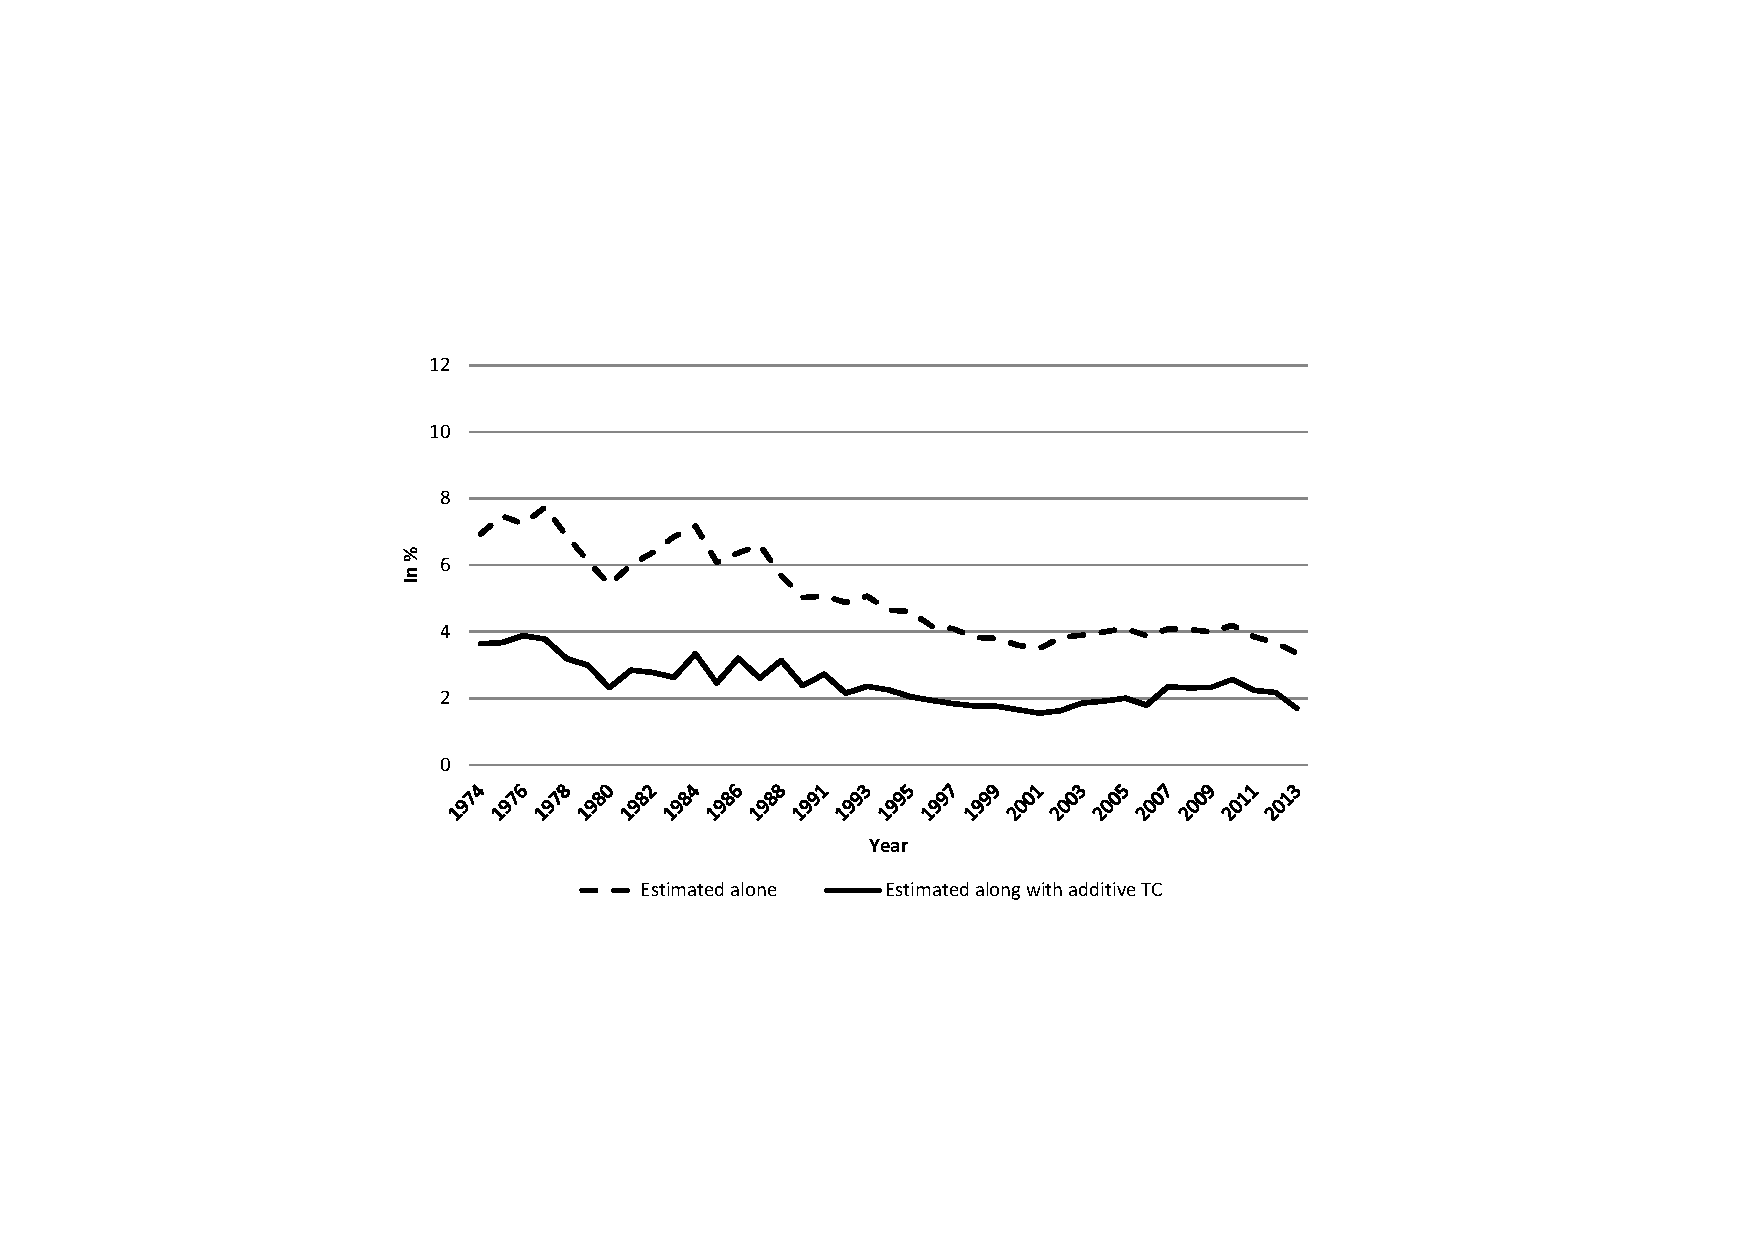
\includegraphics[width=3in, height=2.5in]{Fig1a_mult_air_3d.pdf}
& 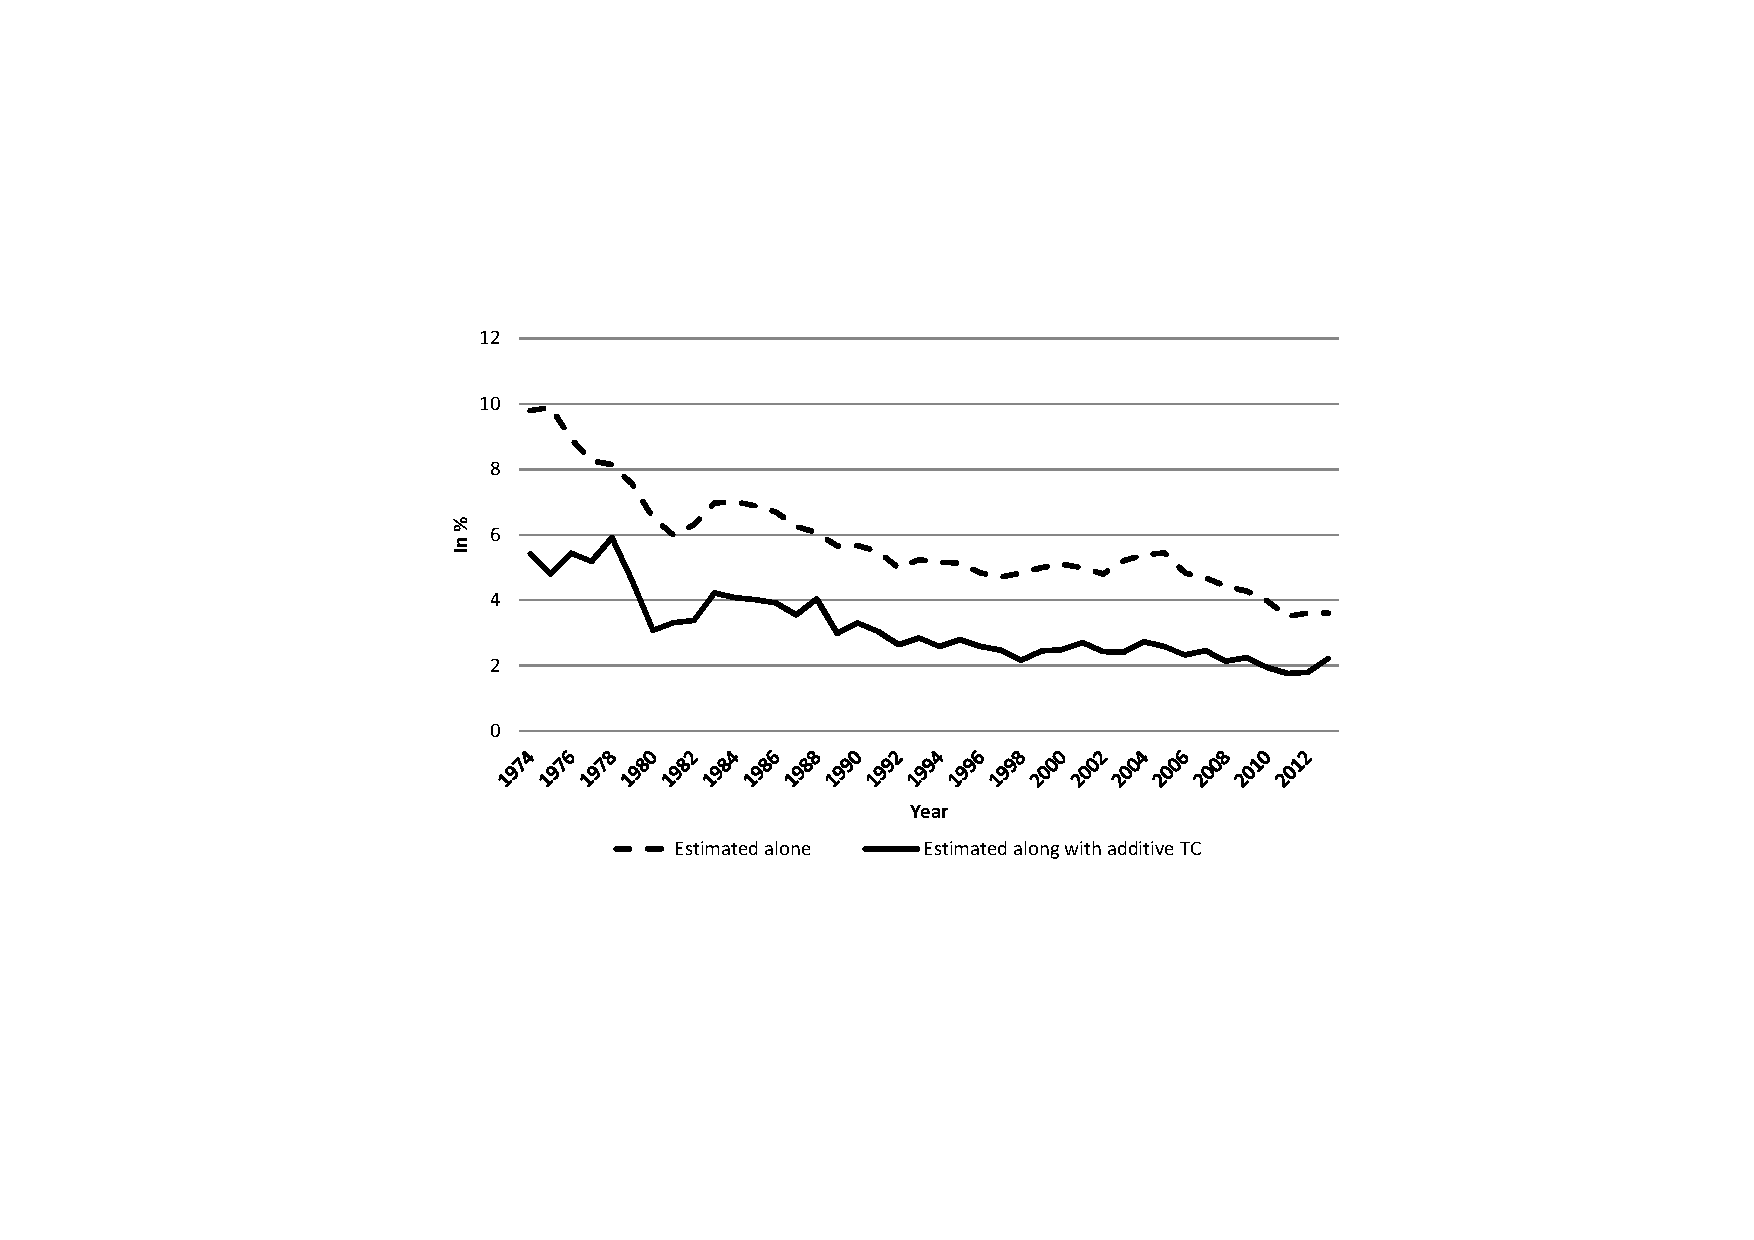
\includegraphics[width=3in,height=2.5in]{Fig1b_mult_vessel_3d.pdf} \\
\end{tabular}
\end{center}
\end{figure}

From Figure \ref{fig:mult_alone_withadd}, we can infer that the sizeable magnitude of additive costs also holds on a yearly basis. Further, Figure \ref{fig:mult_alone_withadd} reports that for Air, the size of the bias seems to decrease over time, while it appears rather stationary for ocean shipping. Put it differently, this suggests that the share of the additive component in total transport costs has decreased over time for air shipping. To get a better picture on this, we study the shares of both ad-valorem and additive components in total costs, by transport mode and over time, based on Figure \ref{fig:decomp_TC_3d}.

\begin{figure}[htbp]
\caption{Decomposing Transport costs (Yearly mean value, 3 digits, in \% of the fas price)}
\label{fig:decomp_TC_3d}
\begin{center}
\begin{tabular}{cc}
{\small (a) Air } & {\small (b) Vessel}\\
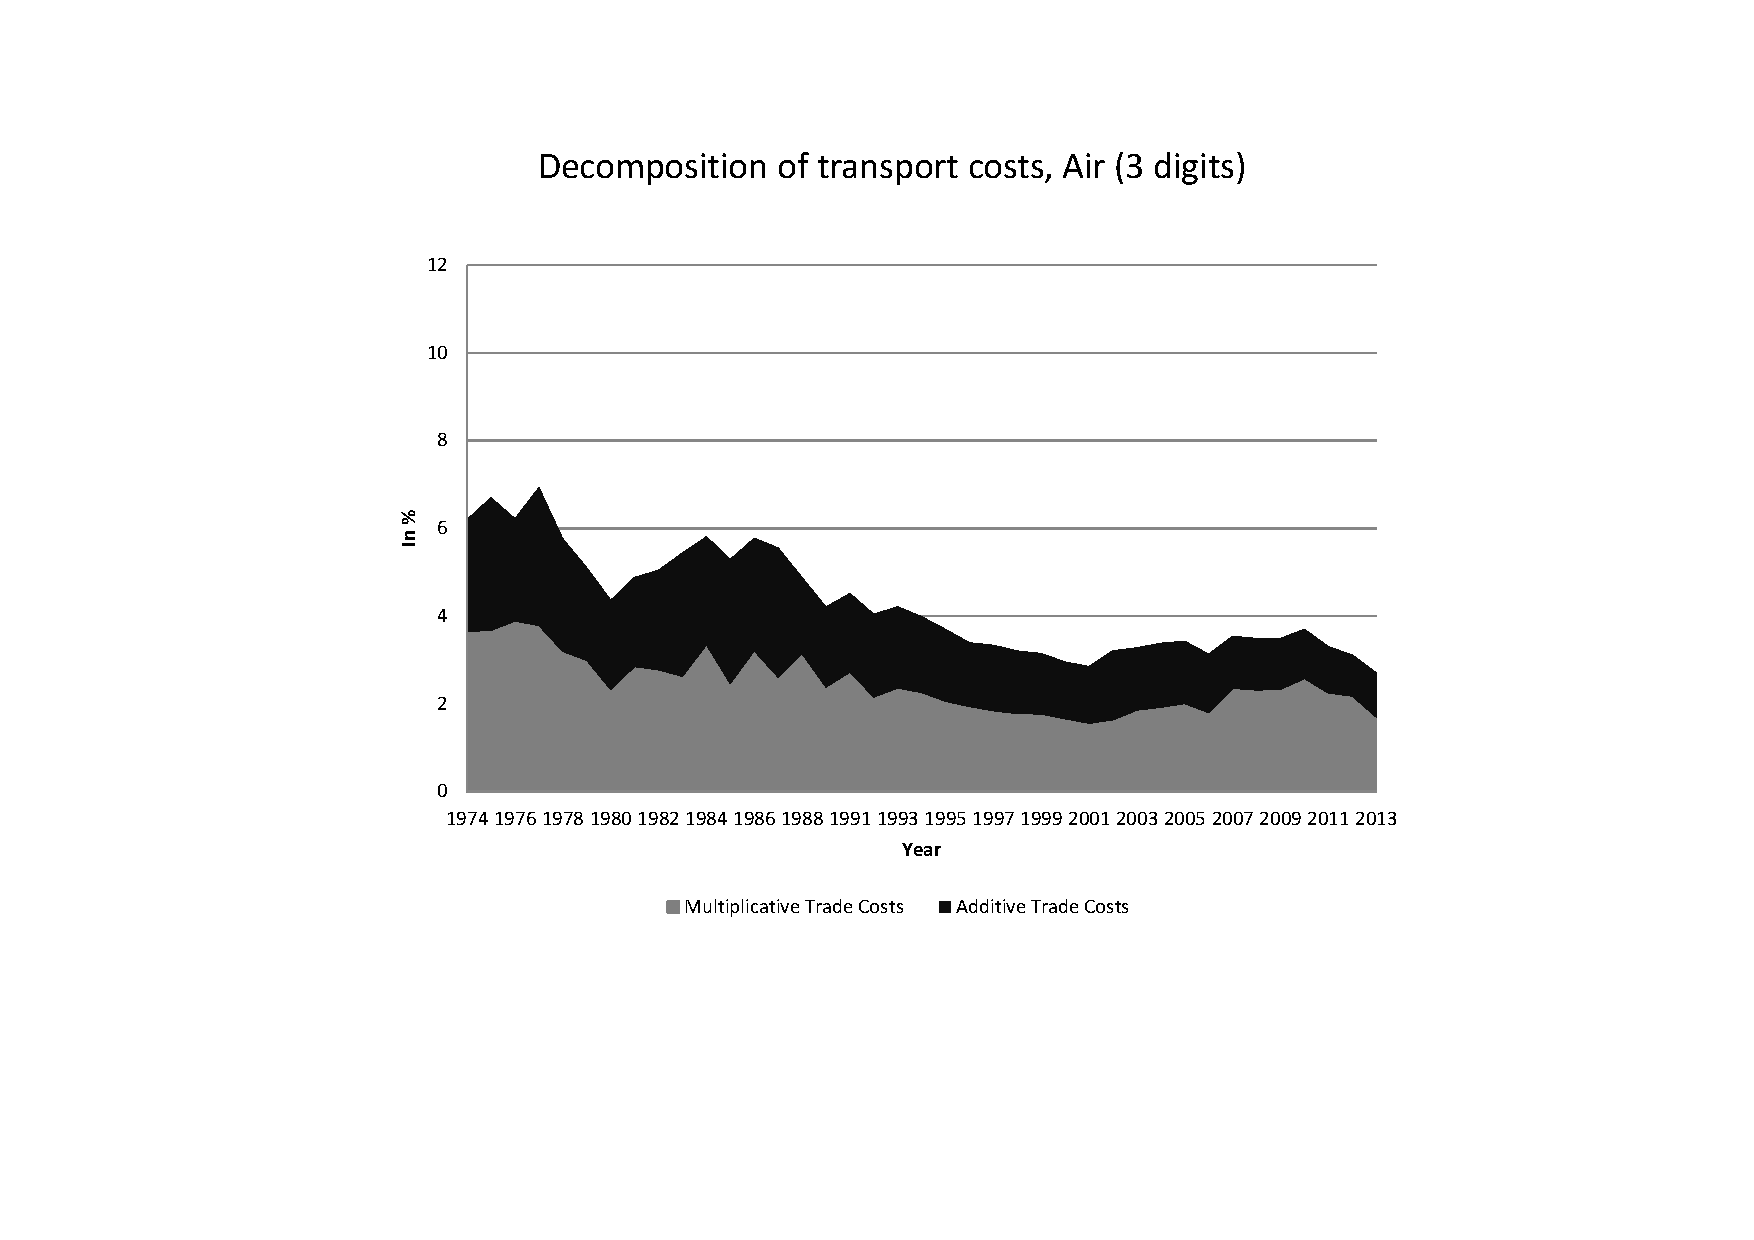
\includegraphics[width=3in, height=2.5in]{Fig2a_decompTC_air_3d.pdf}
& 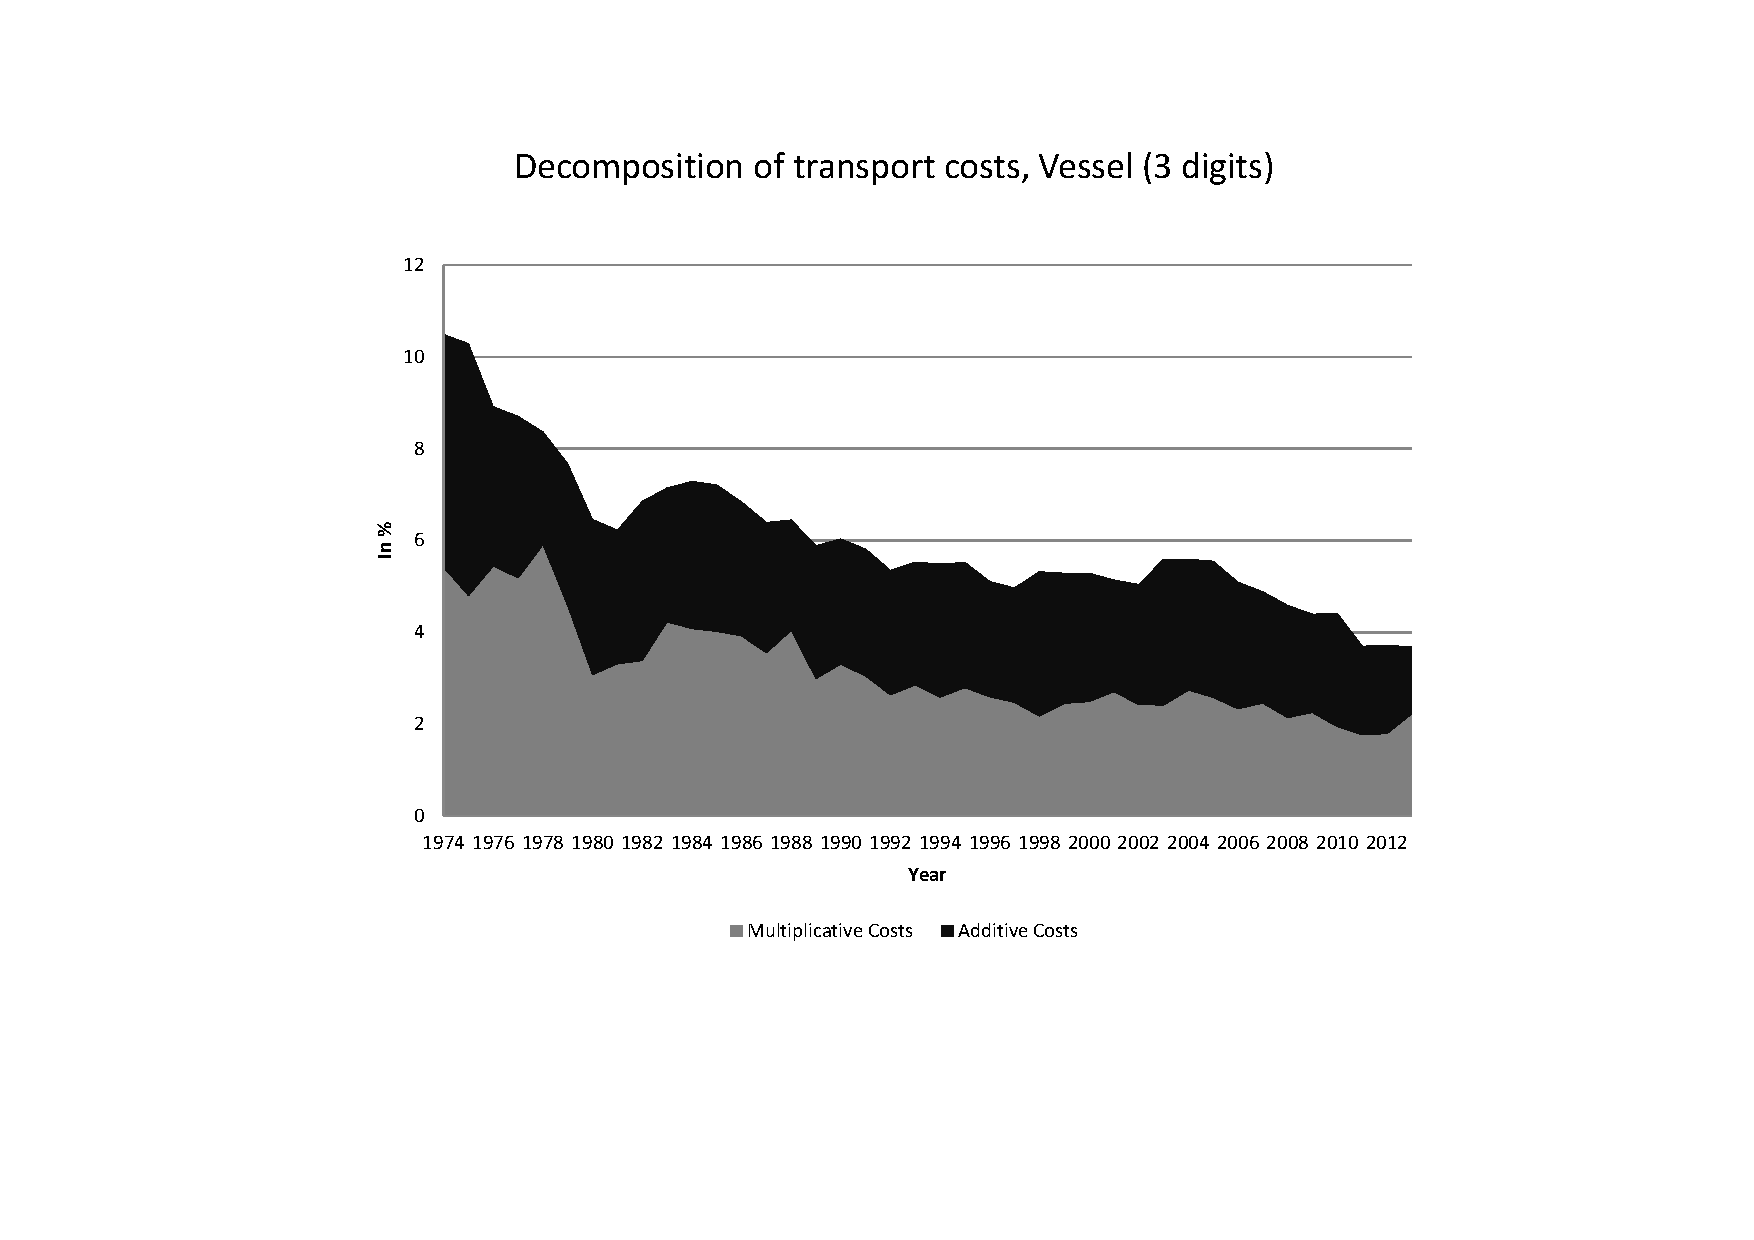
\includegraphics[width=3in,height=2.5in]{Fig2b_decompTC_vessel_3d.pdf} \\
\end{tabular}
\end{center}
\end{figure}


The overall trend pictured in these estimates is in line with the findings by \citet{Hummels_1999}, who point that the overall transport cost for the United States declined from 6 percent to 4 percent between 1974 and 1996. For the same years, our own results point to a total decrease from 6.9 to 4.2\% on average for air shipping, and from 9.8\% to 4.8\% for ocean shipping.\footnote{One may be puzzled for by the high magnitude of estimates for the beginning of the period (say, until 1980) for Ocean transport. \citet{hummels2007} finds similar outcomes on tramp prices indexes, and suggests the oil shock as a likely culprit, in a context where technological progress was quicker in aviation than in vessel, allowing a better dampening of oil shocks on freight rates.} Once again, the fact that our estimates are on average higher than those by \citet{Hummels_1999} should not be a surprise, since ours are simple averages, whereas \citet{Hummels_1999}'s are trade-weighted. But the fact that trends are very close are comforting. It appears therefore that the magnitude of transport costs is higher for ocean shipping than for air shipping.

Besides, we go beyond by distinguishing within these evolutions between multiplicative and additive transport costs. First, the decreasing trend holds considering ad-valorem costs alone (Figure \ref{fig:mult_alone_withadd}), as well as in presence of additive costs (Figure \ref{fig:decomp_TC_3d}), for all years throughout the period. Second, in both transport modes, the additive component appears of sizeable importance. As mean value over the period, it amounts to 48.2\% of total transport costs in Vessel, and 42.3\% in Air. We go on investigating this result further in the next subsection.\footnote{Figure \ref{fig:decomp_TC_3d} also delivers interesting results with respect to the time trends of transport costs. We come back to this aspect in Section \ref{sec:results_trends}.}

Before, we check how our estimates of additive costs compare to those of \citet{Irrazabal_2015}, which provide the most recent evidence on that matter. Based on Norwegian firm-level trade data for 2004, \citet{Irrazabal_2015} find that additive costs are on average 14\% of the median price. Expressed in our own terminology, this means they find that $\frac{t/\tau}{\widetilde{p}}=14\%$. Let us define the ratio of additive costs over total costs as $\frac{t}{\tau\widetilde{p}+t}$, and divide both numerators and denominators by $\tau\widetilde{p}$. We get: $\frac{t}{\tau\widetilde{p}+t}=\frac{t/\tau\widetilde{p}}{1+t/\tau\widetilde{p}}$. Plugging \citet{Irrazabal_2015} result gives 0,14/1+0,14= 12,5\%. Additive trade costs represents 12.5\% of total trade costs. Based on \citet{anderson_wincoop_jel}, we know that transport costs represent a 11\% markup over production costs, and that total international trade costs represent 74\%, so transport costs amount to 11/74= 15\% of total trade costs. Given that in 2004, our estimates for additive (multiplicative) transport costs is 2.9\% (2.7\%) for Vessel, the same reasoning as before leads to 2.9/(2.7+2.9)*11/74 = 7.7\% of total trade costs, that is 62\% (7.7/12.5=62\%) of \citet{Irrazabal_2015}'s estimates. For Air transportation, our estimates for additive (multiplicative) transport costs is 1.5\% (1.9\%), and the same computation brings that additive costs represent 6.6\% of total trade costs, that is 53\% of \citet{Irrazabal_2015}'s estimates. In other words, we find that additive transport costs represent between half and two thirds of the total additive trade costs, which seems totally consistent with the magnitudes reported by e.g. \citet{anderson_wincoop_jel}.


\subsection{Assessing the importance of additive transport costs}

In this section, we explore the performances of each type of model (with and without additive costs) in fitting the observed cif-fas prices gap, in order to deliver a more systematic diagnosis about the importance of additive costs. To do so, we rely on several standard measures of fit. The first indicator is through comparing $R^{2}$. However, its use is far from being straightforward when evaluating non-linear estimates.\footnote{$R^2$ is based on the underlying assumption that the adjusted model is a linear one. In a non-linear context, $R^2$ is  strictly speaking inappropriate. However, if the error distribution is approximately normal, a standard metric like $R^2$ remains informative on the quality of adjustment.} This drives us to complement the goodness of fit diagnosis with three alternative measures. We provide the Standard Error of Regression (SER), which represents the average distance that the observed values fall from the regression line. Smaller values are better because it indicates that the observations are closer to the fitted line. We also report the log-likelihood function, and two measures derived, the Akaike Information Criterion (AIC) and the log-likelihood (LL) ratio test. A decrease in the log-likelihood function points to a better quality-of-fit. However, the likelihood function systematically decreases with the number of parameters included; the AIC criterion allows for correcting this overfitting by including a penalty in the computation of the statistic.\footnote{Precisely, the AIC stat is equal to $2 \times \textrm{number of parameters} - 2 \times \textrm{Likelihood} $.} The preferred model is the one with the minimum AIC value. Finally, the log-likelihood ratio test statistic compares systematically the likelihood of the Unrestricted model (\emph{UR}, including an additive term, i.e. Equation (\ref{eq:model_IetA}) and the Restricted one (\emph{R}, i.e. Equation (\ref{eq:model_nlI})). The null tested is that the two models are statistically equivalent. Results are reported in Tables \ref{tab:good_fit_air} and \ref{tab:good_fit_vessel}, for Air and Vessel respectively, at the 3-digit level.\footnote{Due to our time coverage, we do not report the results for all years (at the 3-digit level). The results for all years are available upon request to the authors.}\medskip



\begin{table}[htbp]
  \centering
  \caption{Air: Measures of Goodness-of-fit (3 digits)}
  \footnotesize{
\begin{center}
    \begin{tabular}{l|cccccc|c}
    \hline \hline
    Year  & 1974  & 1980  & 1990  & 2000  & \multicolumn{1}{c}{2010} & \multicolumn{1}{c}{2013} & Mean stat \\ \hline
    \multicolumn{8}{l}{\bf{$R^2$} }\\ \hline
    Term I only & 0.30  & 0.27  & 0.25  & 0.32  & \multicolumn{1}{c}{0.42} & \multicolumn{1}{c}{0.34} & 0.31 \\
    Terms A \& I & 0.59  & 0.65  & 0.63  & 0.64  & \multicolumn{1}{c}{0.51} & \multicolumn{1}{c}{0.46} & 0.60 \\ \hline
    \multicolumn{8}{l}{\textbf{SER}  }  \\ \hline
    Term I only & 0.79  & 0.86  & 0.81  & 0.84  & \multicolumn{1}{c}{0.86} & \multicolumn{1}{c}{0.92} & 0.85 \\
    Terms A \& I & 0.67  & 0.71  & 0.67  & 0.70  & \multicolumn{1}{c}{0.79} & \multicolumn{1}{c}{0.85} & 0.73 \\ \hline
   \multicolumn{8}{l}{\textbf{AIC criteria}}  \\ \hline
    Term I only & 35674.98 & 41170.98 & 60715.58 & 87492.55 & \multicolumn{1}{c}{102297.66} & \multicolumn{1}{c}{88191.87} & 70498.1 \\
    Terms A \& I & 31387.29 & 35738.39 & 52098.91 & 74954.88 & \multicolumn{1}{c}{95887.05} & \multicolumn{1}{c}{80873.72} & 62285.0 \\ \hline
    \multicolumn{8}{l}{\textbf{Log-likelihood}} \\ \hline
    Term I only & -17530.5 & -20253.5 & -29977.8 & -43341.3 & \multicolumn{1}{c}{-50746.8} & \multicolumn{1}{c}{-43692.9} & -34888.6 \\
    Terms A \& I & -15125.6 & -17263.2 & -25393.5 & -36788.4 & \multicolumn{1}{c}{-47277.5} & \multicolumn{1}{c}{-39751.9} & -30508.3 \\
    LL ratio & 4809.7 & 5980.6 & 9168.7 & 13105.7 & \multicolumn{1}{c}{6938.6} & \multicolumn{1}{c}{7882.1} & 8760.69 \\
    nb of restrictions & 355   & 369   & 393   & 426   & \multicolumn{1}{c}{426} & \multicolumn{1}{c}{427} & 402 \\
    p-value & 0.00 & 0.00 & 0.00 & 0.00 & \multicolumn{1}{c}{0.00} & \multicolumn{1}{c}{0.00} & 0.00 \\
    \hline \hline
 \end{tabular}%
    \end{center}}
  \label{tab:good_fit_air}%
 \parbox[l]{12cm}{\tiny{Notes: SER = Standard Error of regression; AIC = Akaike Information Criterion. $R^{2}$ between the log of predicted ratio and the log of the observed ratio. For the LL ratio test, the number of restrictions is equal to the number of parameters estimated, i.e., the number of partner countries plus the number of products. The mean statistics calculated as the average value over all years. }}
\end{table}%

\begin{table}[htbp]
  \centering
  \caption{Vessel: Measures of Goodness-of-fit (3 digits)}
    \footnotesize{
\begin{center}
\begin{tabular}{l|cccccc|c}
\hline \hline
Year  & \multicolumn{1}{c}{1974} & \multicolumn{1}{c}{1980} & \multicolumn{1}{c}{1990} & \multicolumn{1}{c}{2000} & 2010  & \multicolumn{1}{c}{2013} & Mean stat \\ \hline
\multicolumn{8}{l}{\bf{$R^2$} }\\ \hline
Term I only & \multicolumn{1}{c}{0.450} & \multicolumn{1}{c}{0.415} & \multicolumn{1}{c}{0.456} & \multicolumn{1}{c}{0.401} & 0.350 & \multicolumn{1}{c}{0.339} & 0.39 \\
Terms A \& I & \multicolumn{1}{c}{0.612} & \multicolumn{1}{c}{0.575} & \multicolumn{1}{c}{0.590} & \multicolumn{1}{c}{0.571} & 0.491 & \multicolumn{1}{c}{0.462} & 0.56 \\ \hline
\multicolumn{8}{l}{\textbf{SER}  }  \\ \hline
    Term I only & \multicolumn{1}{c}{0.58} & \multicolumn{1}{c}{0.62} & \multicolumn{1}{c}{0.59} & \multicolumn{1}{c}{0.65} & 0.74  & \multicolumn{1}{c}{0.76} & 0.66 \\
    Terms A \& I & \multicolumn{1}{c}{0.48} & \multicolumn{1}{c}{0.53} & \multicolumn{1}{c}{0.51} & \multicolumn{1}{c}{0.55} & 0.66  & \multicolumn{1}{c}{0.68} & 0.57 \\ \hline
   \multicolumn{8}{l}{\textbf{AIC criteria}}  \\ \hline
    Term I only & \multicolumn{1}{c}{33328.8} & \multicolumn{1}{c}{33010.3} & \multicolumn{1}{c}{51142.6} & \multicolumn{1}{c}{71365.9} & 84789.9 & \multicolumn{1}{c}{88191.9} & 57848.6 \\
    Terms A \& I & \multicolumn{1}{c}{27331.5} & \multicolumn{1}{c}{28067.3} & \multicolumn{1}{c}{43664.7} & \multicolumn{1}{c}{60475.9} & 76161.3 & \multicolumn{1}{c}{80873.7} & 49682.3 \\ \hline
    \multicolumn{8}{l}{\textbf{Log-likelihood}} \\ \hline
    Term I only & \multicolumn{1}{c}{-16287.4} & \multicolumn{1}{c}{-16129.1} & \multicolumn{1}{c}{-25169.3} & \multicolumn{1}{c}{-35263.9} & -41998.9 & \multicolumn{1}{c}{-43692.9} & -28534.3 \\
    Terms A \& I & \multicolumn{1}{c}{-12985.8} & \multicolumn{1}{c}{-13353.7} & \multicolumn{1}{c}{-21171.4} & \multicolumn{1}{c}{-29491.0} & -37418.7 & \multicolumn{1}{c}{-39751.9} & -24151.3 \\
    LL ratio & \multicolumn{1}{c}{6603.28} & \multicolumn{1}{c}{5550.96} & \multicolumn{1}{c}{7995.88} & \multicolumn{1}{c}{11545.98} & 9160.56 & \multicolumn{1}{c}{7882.15} & 8766.0 \\
    nb of restrictions & \multicolumn{1}{c}{393} & \multicolumn{1}{c}{395} & \multicolumn{1}{c}{411} & \multicolumn{1}{c}{436} & 424   & \multicolumn{1}{c}{427} & 417 \\
    p-value& \multicolumn{1}{c}{0.00} & \multicolumn{1}{c}{0.00} & \multicolumn{1}{c}{0.00} & \multicolumn{1}{c}{0.00} & 0.00  & \multicolumn{1}{c}{0.00} & 0.00 \\
    \hline \hline
    \end{tabular}%
    \end{center}}
  \label{tab:good_fit_vessel}%
  \parbox[l]{12cm}{\tiny{Notes: SER = Standard Error of regression; AIC = Akaike Information Criterion. $R^{2}$ between the log of predicted ratio and the log of the observed ratio. For the LL ratio test, the number of restrictions is equal to the number of parameters estimated, i.e., the number of partner countries plus the number of products. The mean statistics calculated as the average value over all years. }}
\end{table}%


Tables \ref{tab:good_fit_air} and \ref{tab:good_fit_vessel} lead to the same conclusion: The inclusion of the additive term leads to an improvement of the quality of fit, whatever the considered criterion or the transport mode. On average over the whole period, the $R^{2}$ doubles when per-kg costs are included for Air, and increases by 50\% for Vessel. Similar qualitative conclusions arise from the comparisons of the standard errors of the regression (SER). Regarding the other criteria, improvements allowed by the inclusion of the additive term are roughly of the same extent across transport modes. Both AIC and Log-Likelihood statistics decrease with the inclusion of the additive term, and the log-likelihood test unambiguously rejects the null of statistical equivalence of the two models. These results holds whatever the considered year.\smallskip


For comparison purposes, we provide a similar goodness-of-fit exercise at the 4-digit product level (4-digits), reported in in Appendix \ref{app:robust_4d}, Tables \ref{tab:good_fit_air_rob} and \ref{tab:good_fit_ves_rob}. If anything, the quality of fitting appears slightly higher when estimations are based on the 4-digit classification. This is especially true for the model restricting trade cost to their ad-valorem dimension, whatever the transport mode considered. When the additive part is taken into account however, the difference in goodness of fit between the 3- and the 4-digit classification level becomes very small, whatever the considered criterion. In other words, if using a more disaggregated classification unsurprisingly adds some statistical precision, this is not with an extent that would disqualify the use of slightly more aggregated data. Further, the same conclusion established at the 3-digit level regarding the significant role of the additive components in fitting international transport costs emerges at the 4-digit level.



\section{Decomposing Transport Costs: Characterizing the trends }\label{sec:results_trends}
\subsection{Estimation strategy}
In this section, we investigate the role of the additive component in total transport costs in a historical perspective.
As a first step, we come back to Figure \ref{fig:decomp_TC_3d}, which displays the respective shares of additive and iceberg components in transport costs over time by transport mode. Considering the trend in total transport costs (the upper line in Figure \ref{fig:decomp_TC_3d}), both air and ocean shipping exhibit a downward trend in overall transport costs since 1974 (-2.1\% per year for mean air transport costs and -2.0\% per year for mean ocean transport costs).\footnote{One may worry that this result springs from high oil-shock related transport costs in 1974. However, computing the time trends from 1980 does not dramatically change the picture. The yearly trend from 1980 is -2\% for mean air transport costs and -1.6\% for mean ocean transport costs. We thus choose to exploit the whole time dimension of our database by taking 1974 as starting date of our time trend analysis.}

Before making any definite statement about this though, it is worth emphasizing that the time trend of international transport costs depends on both \textit{i)} the evolution of per product and per partner transport costs and \textit{ii)} the evolution of the composition of trade. Total transport costs may thus have decreased over time because the share of neighbor countries in total US trade or the share of goods cheaper to transport has increased (explanation \textit{ii)}), independently of any change in transport costs \textit{per se}. As argued by \cite{hummels2007}, it is hence necessary to eliminate the composition effects of trade flows to isolate the evolution of ``pure'' international transport costs, i.e. per product- and per partner- transport costs.


If we share this view with \cite{hummels2007}, we adopt a different strategy for eliminating composition effects, which builds upon our first-stage results.\footnote{See Appendix for a detailed comparison of Hummel's (2007) methodology and ours.} Estimation driven in Section \ref{sec:results_decomposition} indeed provides us with the two additive and ad-valorem measures of international transport costs (Equation (\ref{eq:estimatedequation})), that vary over time, product and origin country. Starting from these values, we extract the ``pure'' transport cost component (additive and multiplicative, by transport mode) by the mean of a time fixed effect (see details below). By comparing the additive cost component unfitted (total) and fitted (composition effects excluded), we characterize if this dimension of the transport cost has fallen due to (for instance) the fact that product quality has increased over time (weight has reduced, hence reducing the transport cost by dollar transported), or if it is the ``pure'' additive costs (for instance, handling costs) that have reduced over time. We proceed similarly for the multiplicative component of trade costs. We also agglomerate the two components (additive and iceberg) in a unified measure of transport costs. This allows us to compare how ``pure'' transport costs have changed over time, composition effects excluded, and to compare them to the unfitted ones.\footnote{Notice that these ``unfitted'' total transport costs are virtually the same as those reported in Figure \ref{fig:decomp_TC_3d}, but reported in another perspective (basis 100 in year 1974).}

Doing so, our empirical analysis differentiates from from \cite{hummels2007} in two main dimensions. First, our characterization of the time trends in transport costs identifies the trend patterns of the ``pure'' transport costs'' (composition effects excluded) for both the additive and ad-valorem costs, as well as for the overall transport cost. Second, our methodology assumes a share between the additive and the ad-valorem components of transport costs, that varies over the three time/product/country partner dimensions. By contrast, \cite{hummels2007} does not take into account the changes in the additive transport cost component, attributing this to a change in the composition of the bundle over time (per country-commodity).\footnote{Rigourously speaking, our methodology also differs from  \citet{hummels2007} with respect to the weighting scheme used to obtain the evolution of the ``pure'' transport costs over time. We discuss this point with more details in Appendix \ref{app:comp-effects}.}

\subsection{Empirical specification}
For the estimated ad-valorem component, we estimate the following equation using OLS:
\begin{eqnarray}
\ln(\widehat{\tau}_{ikt})&=&\delta +\underbrace{\sum_{i \neq \text{ARG}}\alpha_i.\mathbb{1}_i}_{(a)} + \underbrace{\sum_{s(k)\neq \text{011}}\beta_{s(k)}.\mathbb{1}_{s(k)}}_{(b)} + \underbrace{\sum_{t \neq 1974}\gamma_t.\mathbb{1}_t}_{(c)}+\epsilon_{ikt} \label{eq:compeffects_mult}
\end{eqnarray}

\noindent where $\mathbb{1}_i$ and $\mathbb{1}_{s(k)}$ represent country- and sector- fixed effects. We cannot use the same equation for the estimated additive component, as by construction, the sector fixed effect and the country fixed effect are additive rather than multiplicative. We estimate the following equation using non-linear least squares:\footnote{For sake of notational simplicity, we do not distinguish the coefficients associated to the fixed effects between Equations (\ref{eq:compeffects_mult}) and (\ref{eq:compeffects_add}), even if they are specific to the type of transport costs considered (e.g., the series of $\gamma_t$ differs from one estimation to the other).}
%, based on the additive cost series $\widehat{t}_{ikt}$ previously obtained:
\begin{eqnarray}
\ln(\widehat{t}_{ikt})&=&\ln\left( \delta + \underbrace{\sum_{i \neq \text{ARG}}  \alpha_i.\mathbb{1}_i}_{(a)}+\underbrace{\sum_{s(k)}\beta_{s(k)}.\mathbb{1}_{s(k)}}_{(b)}\right) + \underbrace{\sum_{t \neq 1974}\gamma_t.\mathbb{1}_t}_{(c)}+\epsilon_{ikt} \label{eq:compeffects_add}
\end{eqnarray}
As displayed in Equations (\ref{eq:compeffects_mult}) and (\ref{eq:compeffects_add}), the objective is to decompose the estimated transport cost component in three components: the country dimension (Term (a)), the product dimension (Term (b)) and the ``pure transport costs time trend'' (Term (c)). Notice that Equations (\ref{eq:compeffects_mult}) and (\ref{eq:compeffects_add}) preserve our specification of the ad-valorem and additive costs of Equations (\ref{eq:ad-valorem}) and (\ref{eq:add}), as we consider that the iceberg cost is the product of the country of origin and the good dimension, while the additive cost is the sum of the two dimensions.\footnote{In the three estimations (ad-valorem costs alone, ad-valorem costs estimated along with additive, and the additive component), we consider Argentina, the sector 011 and the first year of our dataset 1974, as references for the country-, product and -year dummies.} Both equations are estimated by transport mode.

In this exercise, we are interested in isolating the change in the time dimension of the each transport cost component. From the estimation of Equation (\ref{eq:compeffects_mult}), we built the variable $\Gamma^{adv}_t$, for each year $t\geq 1974$, according to:\footnote{See details in Appendix \ref{app:comp-effects}.}
\begin{equation}
\Gamma^{adv}_t = 100.\frac {\bar{\tau}_{1974}.\exp(\gamma_t)-1} {\bar{\tau}_{1974}-1} \label{eq:comp_effects_adv}
\end{equation}

\noindent with $\bar{\tau}_{1974} = \exp(\delta +\sum_i \alpha_i +\sum_s \beta_s)$ the mean multiplicative transport cost in 1974. In plain words, we measure how these costs have changed over time by blocking the composition of trade flows by product and country partners to the one observed in 1974 (the beginning of our sample). This notably enables us to obtain measures of transport costs that are easily comparable between transport modes and transport costs components.

As for the additive cost, we built the variable $\Gamma^{add}_t$, the reference year being 1974 (ie, with $\gamma_{1974}=0$) according to:
\begin{equation}
\Gamma^{add}_t = 100.\exp(\gamma_t) \label{eq:comp_effects_add}
\end{equation}

\noindent As a result, the three series (for $\Gamma^{adv}_t$ and $\Gamma^{add}_t$) have a straightforward interpretation in percentage changes from the initial value of 100 for $t=1974$.

Last, we rebuild a measure of total transport costs as the sum of the two components (additive and iceberg), on both the ``raw'' (without composition effects excluded) and the ``pure'' estimated transport costs (composition effects excluded, see Appendix \ref{app:comp-effects}).


\subsection{Characterizing the time trends in transport costs}
Figure \ref{fig:totalTC_compeffects_excl} reports the results.\footnote{In Appendix \ref{app:comp-effects}, we report the results at a more disaggregated level, distinguishing between primary and manufacturing goods.} In Panels (a) and (b), we report the time changes of the ad-valorem costs and the additive costs respectively. Panel (c) displays the time changes in the total transport costs (built as the sum of the two components as detailed above). In the three cases, the series are reported as indices, starting from the reference value 100 in 1974 and by transport mode.


\begin{figure}[htbp]
\caption{Transport costs (with and without composition effects)}
\label{fig:totalTC_compeffects_excl}
\begin{center}
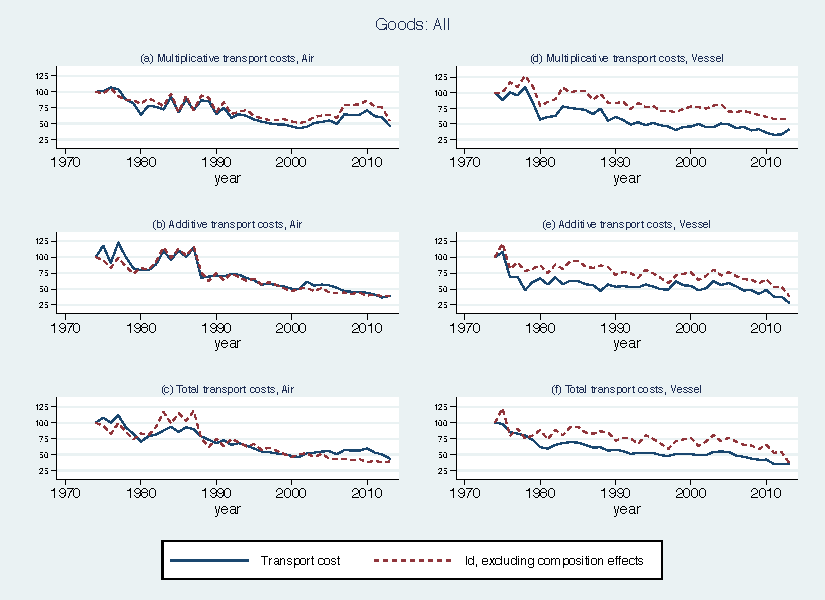
\includegraphics[height=4in]
{graph_composition_all.pdf}
\end{center}
\end{figure}

Three main results emerge from Figure \ref{fig:totalTC_compeffects_excl}. First, echoing the related literature (see \citealp{Lafourcade_Thisse}), we find that international transport costs hae substantially decreased over the period, and in both transport modes. International transport costs were reduced by 50\% between 1974 and 2013 in air shipping, and by 60\% in maritime shipping. Second, the magnitude of the decrease is roughly of same order both the ad-valorem and the additive components. Third, we do not find evidence of a significant difference between the raw transport costs and the ``pure'' transport costs in Air transport, for both the additive and ad-valorem components (Figure \ref{fig:totalTC_compeffects_excl}, left panels). Air transport costs were reduced by 50\% between 1974 and 2013, and this is mainly attributable to a reduction in the ``pure'' transport costs. Composition effects are more pronounced in ocean transport. Considering the raw series, maritime transport costs have decreased by 60\% over the period, which can be decomposed in a 50\% decrease in transport costs \textit{per se}, and a 10\% reduction that comes from composition effects. Precisely, the role of composition effects is significant for the multiplicative component, whereas the reduction in the additive costs is mostly attributable to changes in ``pure'' additive costs.


This last set of results stands in sharp contrast with \citet{hummels2007}, which obtained that the ``pure'' transport costs had decreased more than the unfitted ones (over 1973-2004), suggesting an important role to composition effects. If anything, we find the opposite result here. Investigating this difference of result further (see Appendix \ref{app:comp-effects}), we find that this can be explained by the difference in methodology, and primarily the treatment of the additive component transport costs. Assuming a varying share of the additive component over time, product and country partner indeed modifies the decomposition of the trend reduction of transport costs between the one attributable to trade composition effects and the reduction in the ``pure'' transport costs. In both air and ocean transports, we thus find that this last dimension is the main driver of the reduction of international transport costs observed over time, in particular in ocean transport.



\section{Robustness checks \label{sec:robustness}}

Robustness to the specification of the estimated equation.

\paragraph{Robustness to the separability assumption}


Ie, estimate


$$\log(\frac{p_{ik}}{\widetilde{p}_{ik}} -1)= \log(\tau_{is} -1+ \frac{t_{is}}{\widetilde{p}_{ik}})+ \exp(\epsilon_{ik})$$

To do on 100 products ($s$), 50 countries (the most important?)

\todo{what else?}

\section{Conclusion \label{sec:conclu}}

This paper empirically studies the magnitude of additive (or per-kg) costs in international transport costs, by exploiting the differences between the import and the export prices. Using SITC 3 and 4- digit cif-fas unit values taken from the US import database over 1974-2013, we estimate the two components of transport costs, by transport mode (air or ocean).  Our results may be summarized in three main findings. First, we provide a quantitative measure of both the additive and the iceberg transport cost. We thus find that additive costs amount to 2.8\% of the export price unit values for ocean shipping, and ad-valorem ones 3.2\%. These values are respectively equal to 1.8 and 2.5\% for air transport. Second, we show that taking additive costs into account improves the fit of the modelling of transport costs. All goodness-of-fit measures point out to this conclusion, which holds for both transport modes and all years considered. Third, we also use the time dimension of our data to characterize the evolution of transport costs. [...] \textbf{completer} In all three aspects, our results point the importance of the additive component in accounting for international transport costs.

Our results could be extended in two main ways. On the empirical side, one may want to ge deeper in the ``structural'' determinants of trade costs, i.e. identify the respective roles of handling costs, insurance and freight at the root of the gap between export and import prices. On the theoretical side, our results can be used to explore the role of additive costs in shaping international trade flows (in an international trade theory perspective) and in affecting the international transmission of business cycles. This is left for further research.



\newpage
\bibliographystyle{essaien}
\bibliography{biblio}


\newpage


\appendix

\section{Data Appendix \label{app:data}}


The Customs value is the value of imports as appraised by the U.S. Customs and Border Protection in accordance with the legal requirements of the Tariff Act of 1930, as amended. This value is generally defined as the price actually paid or payable for merchandise when sold for exportation to the United States, excluding U.S. import duties, freight, insurance, and other charges incurred in bringing the merchandise to the United States. The term ``price actually paid or payable'' means the total payment (whether direct or indirect, and exclusive of any costs, charges, or expenses incurred for transportation, insurance, and related services incident to the international shipment of the merchandise from the country of exportation to the place of importation in the United States) made, or to be made, for imported merchandise by the buyer to, or for the benefit, of the seller. In this respect, the ``custom value'' corresponds to the fas price (``free-alongside'' price) delivered by the seller.

The import charges represent the aggregate cost of all freight, insurance, and other charges (excluding U.S. import duties) incurred in bringing the merchandise from alongside the carrier at the port of exportation in the country of exportation and placing it alongside the carrier at the first port of entry in the United States. In the case of overland shipments originating in Canada or Mexico, such costs include freight, insurance, and all other charges, costs and expenses incurred in bringing the merchandise from the point of origin (where the merchandise begins its journey to the United States in Canada or Mexico to the first port of entry.

The cif (cost, insurance, and freight) value represents the landed value of the merchandise at the first port of arrival in the United States. It is computed by adding ``Import Charges'' to the ``Customs Value'' (see definitions above) and therefore excludes U.S. import duties.

\section{Estimation at the 3-digit classification level \label{app:more_results}}

\subsection{Transport costs estimates: More detailed results}

In this section, we report more detailed results for the estimates for international transport costs, by transport mode on a yearly basis, when either additive costs are included in the estimation (Equation (\ref{eq:model_IetA})) or not (Equation (\ref{eq:model_nlI})), under our benchmark sectoral classification level (3 digit). Precisely, we complement the results displayed in Table \ref{tab:summary_results} by reporting the estimates of international transport costs for a sample of years over 1974-2013, when the degree of classification retained ($s$) is at the 3-digit classification level. Table \ref{tab:result_air_3d_detail} reports the results for Air transport. The results for Ocean transport are displayed in Table \ref{tab:result_ves_3d_detail}.

\todo{Changer la facon de presenter les resultats, pour harmoniser avec la facon de faire dans le corps du papier. Jerome?}
\begin{table}[htbp]
  \centering
  \caption{Air: Transport costs estimates, 3-digits (selected years)}
\begin{center}
    \begin{tabular}{l|cccccc}
\hline\hline

Year & 1974  & 1980  & 1990  & 2000  & 2010  & 2013   \\ \hline
\multicolumn{7}{l}{\textbf{With only Iceberg Trade Costs}}     \\ \hline
Mean  & 1.069 & 1.054 & 1.050 & 1.036 & 1.042 & 1.034  \\
Median & 1.054 & 1.038 & 1.044 & 1.025 & 1.034 & 1.029  \\
Standard Error & 0.052 & 0.049 & 0.039 & 0.033 & 0.037 & 0.024 \\
\hline
\multicolumn{7}{l}{\textbf{With Additive \& Iceberg Trade Costs }}    \\ \hline
\multicolumn{7}{l}{\textit{Additive term }}     \\ \hline
\multicolumn{1}{l}{Mean } & 0.026 & 0.020 & 0.018 & 0.013 & 0.011 & 0.010  \\
\multicolumn{1}{l}{Median} & 0.011 & 0.005 & 0.008 & 0.005 & 0.004 & 0.005  \\
\multicolumn{1}{l}{Standard Error} & 0.040 & 0.041 & 0.033 & 0.028 & 0.024 & 0.020  \\ \hline
\multicolumn{7}{l}{\textit{Iceberg term}}  \\ \hline
\multicolumn{1}{l}{Mean } & 1.036 & 1.023 & 1.024 & 1.017 & 1.026 & 1.017  \\
\multicolumn{1}{l}{Median} & 1.027 & 1.016 & 1.016 & 1.012 & 1.022 & 1.017 \\
Standard Error & 0.032 & 0.025 & 0.021 & 0.016 & 0.023 & 0.012  \\ \hline
\# observations & 14955 & 16118 & 24958 & 35027 & 40279 & 39351  \\
\hline\hline
\multicolumn{7}{l}{\parbox[l]{11cm}{ \vspace{7pt}\scriptsize{Notes: Statistics are obtained weighting each observation by its value in transport (mode-dependent). Additive term expressed in fraction of fas price.}}}
\end{tabular}%
\end{center}
\label{tab:result_air_3d_detail}
\end{table}%


\begin{table}[htbp]
  \centering
  \caption{Vessel: Transport costs estimates, 3 digit (selected years)}
\begin{center}
    \begin{tabular}{l|cccccc}
   \hline\hline
Year         & 1974  & 1980  & 1990  & 2000  & 2010  & 2013   \\
 \hline
   \multicolumn{7}{l}{\textbf{With only Iceberg Trade Costs} }  \\
Mean  & 1.098 & 1.065 & 1.057 & 1.051 & 1.040 & 1.036  \\
Median & 1.096 & 1.055 & 1.046 & 1.049 & 1.036 & 1.033  \\
Standard Error & 0.053 & 0.040 & 0.032 & 0.028 & 0.020 & 0.018  \\
\multicolumn{7}{l}{\textbf{With Additive \& Iceberg Trade Costs} }    \\
\hline
\multicolumn{7}{l}{\textit{Additive term } }  \\ \hline
Mean  & 0.051 & 0.034 & 0.027 & 0.028 & 0.025 & 0.015  \\
Median & 0.029 & 0.023 & 0.017 & 0.022 & 0.019 & 0.008 \\
Standard Error & 0.085 & 0.046 & 0.040 & 0.043 & 0.025 & 0.020 \\ \hline
\multicolumn{7}{l}{\textit{Iceberg term} } \\ \hline
Mean  & 1.054 & 1.031 & 1.033 & 1.025 & 1.019 & 1.022 \\
Median & 1.049 & 1.024 & 1.028 & 1.021 & 1.018 & 1.018  \\
Standard Error & 0.041 & 0.023 & 0.022 & 0.021 & 0.018 & 0.018  \\
\hline
 \# obs & 19007 & 17356 & 28383 & 36090 & 37748 & 38473 \\ \hline
\hline\hline
\multicolumn{7}{l}{\parbox[l]{11cm}{ \vspace{7pt}\scriptsize{Notes: Statistics are obtained weighting each observation by its value in transport (mode-dependent). Additive term expressed in fraction of fas price.}}}
\end{tabular}%
\end{center} \label{tab:result_ves_3d_detail}
\end{table}%


\subsection{Variance decomposition exercise \label{app:decomp_variance}}

In this section, we provide a variance decomposition exercise on the observed cif-fas price gap. Precisely, we determine the share of the observed variance in the ratio $\ln(\frac{p_{ik}}{\widetilde{p}_{ik}}-1)$ that comes from \textit{i)} the between-product variance (at the 5-digit level, $k$), \textit{ii)} the between-sector variance (at the 3-digit level, $s$). This gives us an alternative way to ensure the robustness of the estimation results to the degree of classification retained to estimate international transport costs. We also determine the share of the observed variance that can be attributed to the between-country variance. Results are reported in Figure \ref{fig:decomp_variance}.

\begin{figure}[htbp]
\caption{Variance decomposition (observed cif-fas price gap)}
\label{fig:decomp_variance}
\begin{center}
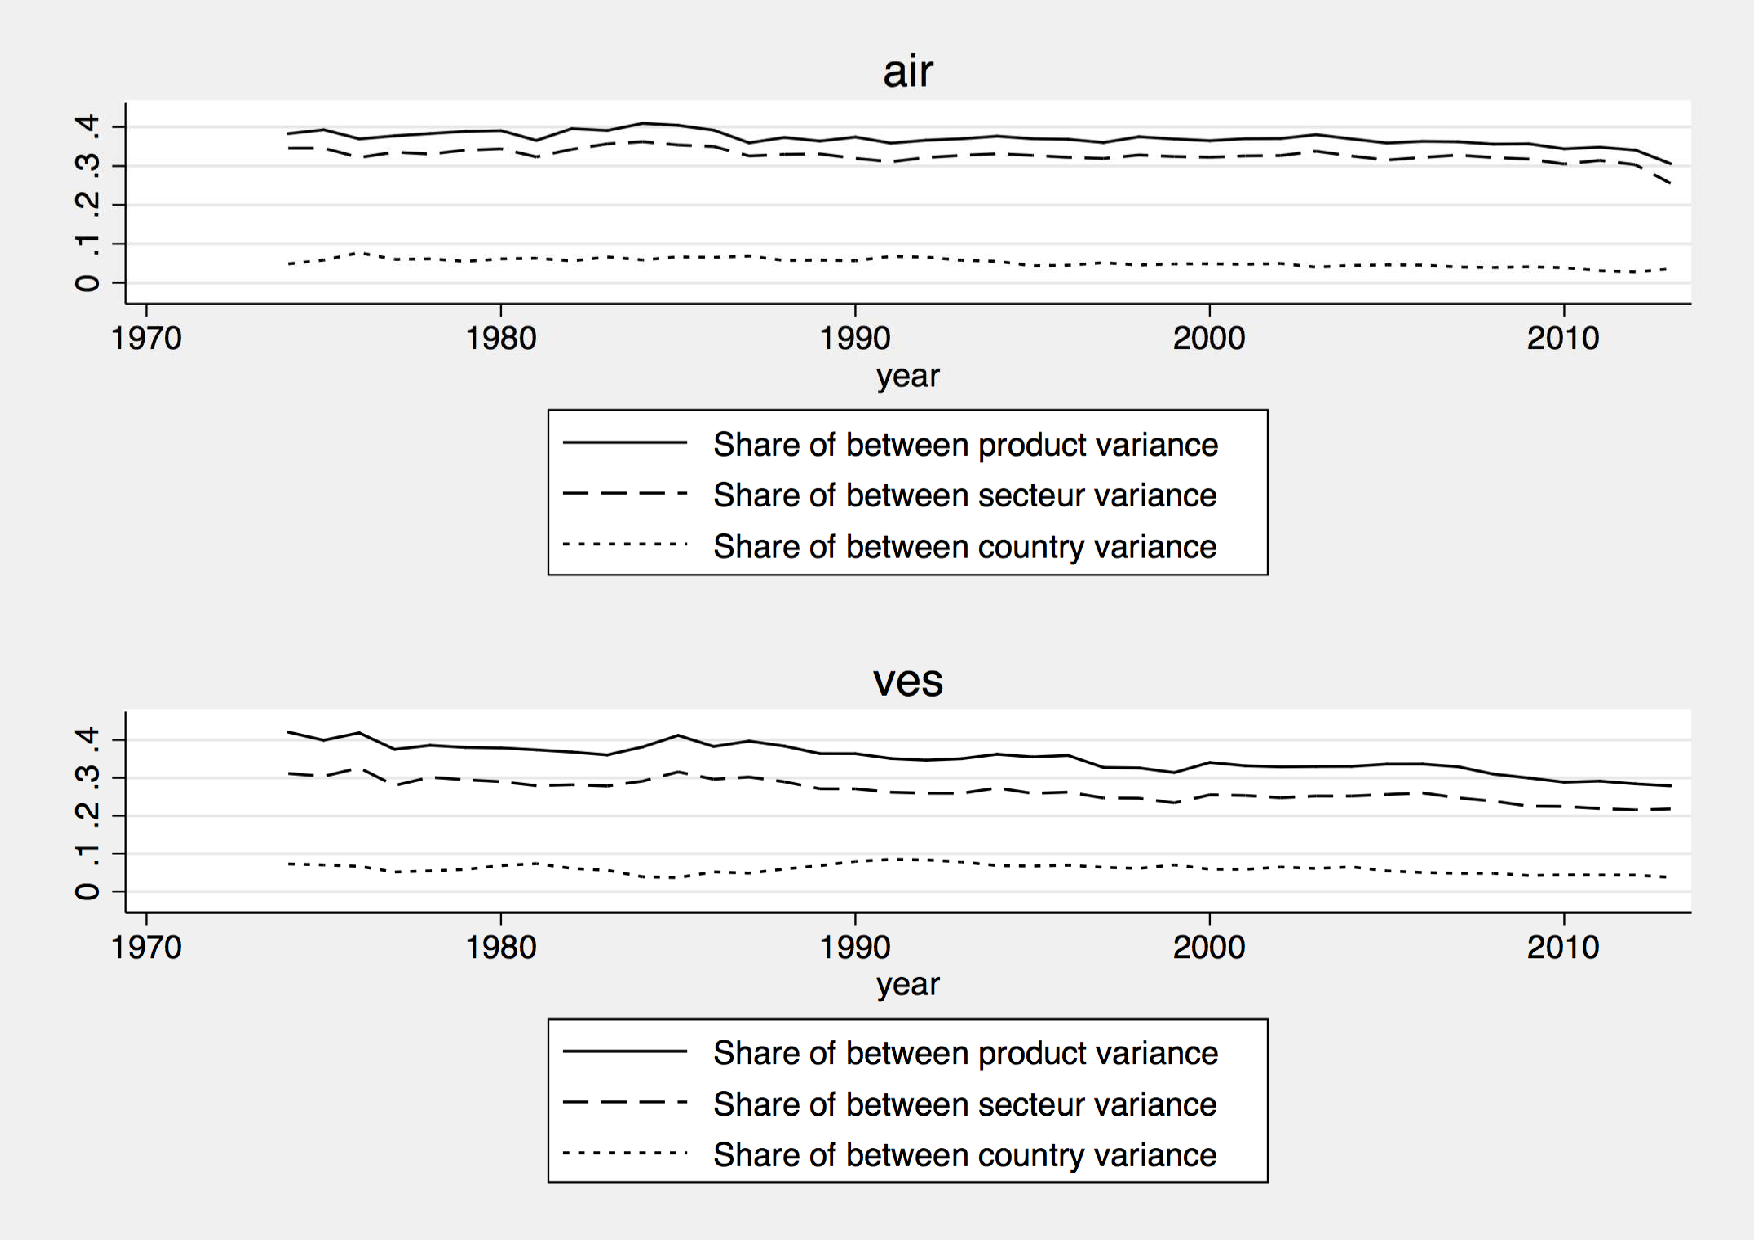
\includegraphics[width=10cm, height=7cm]{variance_decomposition.pdf}
%{\footnotesize {OECD data} }
\end{center}
\end{figure}

Two interesting results emerge from Figure \ref{fig:decomp_variance}. First, the share of the cif-fas price gap variance that comes from the variance between products (5-digit level) is of same magnitude of order at the variance between sectors at the 3-digit level. Both account for between 30 and 40\% of the total variance in Air transport, depending on the years considered. This is also the case for Ocean transport, even if the difference between the between-country variance share and the between-sector share is more pronounced (30\% for the between-sector vs 40\% for the between-product variance at the beginning of the period). This delivers an indirect robustness check to the degree of classification we have retained to estimate international transport costs. Second, the variance of the cif-fas price gap that can be attributed to the product (or sector) dimension is much larger that the between-country variance. This holds throughout the period and for both transport modes. This suggests that what primarily matters in international transport costs is mostly attributable to the product per se, rather than to the country where it comes from. By extension, one can expect a limited role of distance and other country-related variables as determinants of transport costs.

\section{Estimation at the 4-digit level \label{app:4digit}}

In this section, we report the estimation results when we retain the 4-digit classification level ($s$=4-digit).

\subsection{Transport cost estimates}


Tables \ref{tab:result_air_rob} and \ref{tab:result_ves_rob} report the estimates of both models (with and without additive costs) in Air and Ocean transport respectively.

\begin{table}[htbp]
  \centering
  \caption{Air: Transport costs estimates, Selected years, 4-digit}
\begin{center}
    \begin{tabular}{l|cccccc}
   \hline\hline
Year & 1974  & 1981  & 1989  & 2001  & 2009  & 2013 \\ \hline
\multicolumn{7}{l}{\textbf{With only Iceberg Trade Costs} }  \\
Mean  & 1.066 & 1.058 & 1.052 & \multicolumn{1}{c}{1.033} & \multicolumn{1}{c}{1.037} & \multicolumn{1}{c}{1.032} \\
Median & 1.052 & 1.044 & 1.041 & \multicolumn{1}{c}{1.021} & \multicolumn{1}{c}{1.027} & \multicolumn{1}{c}{1.026}  \\
Standard Error & 0.056 & 0.054 & 0.046 & \multicolumn{1}{c}{0.040} & \multicolumn{1}{c}{0.036} & \multicolumn{1}{c}{0.025}  \\
\hline
\multicolumn{7}{l}{\textbf{With Additive \& Iceberg Trade Costs }}  \\ \hline
\multicolumn{7}{l}{\textit{Iceberg term} }   \\ \hline
Mean  & 1.035 & 1.026 & 1.031 & \multicolumn{1}{c}{1.015} & \multicolumn{1}{c}{1.021} & \multicolumn{1}{c}{1.016}  \\
Median & 1.025 & 1.017 & 1.019 & \multicolumn{1}{c}{1.010} & \multicolumn{1}{c}{1.017} & \multicolumn{1}{c}{1.014}  \\
Standard Error & 0.036 & 0.028 & 0.030 & \multicolumn{1}{c}{0.021} & \multicolumn{1}{c}{0.024} & \multicolumn{1}{c}{0.015}  \\ \hline
\multicolumn{7}{l}{\textit{Additive term} }   \\ \hline
Mean  & 0.026 & 0.021 & 0.017 & \multicolumn{1}{c}{0.012} & \multicolumn{1}{c}{0.012} & \multicolumn{1}{c}{0.010} \\
Median & 0.012 & 0.006 & 0.006 & \multicolumn{1}{c}{0.005} & \multicolumn{1}{c}{0.004} & \multicolumn{1}{c}{0.004}  \\
Standard Error & 0.039 & 0.042 & 0.033 & \multicolumn{1}{c}{0.027} & \multicolumn{1}{c}{0.029} & \multicolumn{1}{c}{0.019} \\ \hline
\# obs & 14944 & 16844 & 25307 & \multicolumn{1}{c}{35005} & \multicolumn{1}{c}{38475} & \multicolumn{1}{c}{39460}  \\
\hline\hline
\multicolumn{7}{l}{\parbox[l]{11cm}{ \vspace{7pt}\scriptsize{Notes: Statistics are obtained weighting each observation by its value in transport (mode-dependent). Additive term expressed in fraction of fas price.}}}
\end{tabular}%
\end{center}
  \label{tab:result_air_rob}
\end{table}%


\begin{table}[htbp]
  \centering
\caption{Vessel: Transport costs estimates, Selected years, 4-digit}
\begin{center}
    \begin{tabular}{l|cccccc}
   \hline\hline
Year & 1974  & 1981  & 1989  & 2001  & 2009  & 2013 \\
\hline
\multicolumn{7}{l}{\textbf{With only Iceberg Trade Costs}} \\
Mean  & 1.098 & 1.061 & \multicolumn{1}{c}{1.058} & \multicolumn{1}{c}{1.051} & \multicolumn{1}{c}{1.042} & \multicolumn{1}{c}{1.036}  \\
Median & 1.094 & 1.051 & \multicolumn{1}{c}{1.048} & \multicolumn{1}{c}{1.045} & \multicolumn{1}{c}{1.038} & \multicolumn{1}{c}{1.031} \\
Standard Error & 0.060 & 0.038 & \multicolumn{1}{c}{0.036} & \multicolumn{1}{c}{0.030} & \multicolumn{1}{c}{0.023} & \multicolumn{1}{c}{0.020} \\
\hline
\multicolumn{7}{l}{\textbf{With Additive \& Iceberg Trade Costs } }\\ \hline
\textit{Iceberg term} &       &       &       &       &       &     \\
Mean  & 1.054 & 1.034 & \multicolumn{1}{c}{1.028} & \multicolumn{1}{c}{1.028} & \multicolumn{1}{c}{1.024} & \multicolumn{1}{c}{1.021}  \\
Median & 1.049 & 1.030 & \multicolumn{1}{c}{1.024} & \multicolumn{1}{c}{1.025} & \multicolumn{1}{c}{1.026} & \multicolumn{1}{c}{1.018} \\
Standard Error & 0.043 & 0.026 & \multicolumn{1}{c}{0.025} & \multicolumn{1}{c}{0.021} & \multicolumn{1}{c}{0.016} & \multicolumn{1}{c}{0.013}  \\
\textit{Additive term} &       &       &       &       &       &     \\
Mean  & 0.046 & 0.026 & \multicolumn{1}{c}{0.031} & \multicolumn{1}{c}{0.024} & \multicolumn{1}{c}{0.021} & \multicolumn{1}{c}{0.015}  \\
Median & 0.029 & 0.013 & \multicolumn{1}{c}{0.019} & \multicolumn{1}{c}{0.015} & \multicolumn{1}{c}{0.013} & \multicolumn{1}{c}{0.008} \\
Standard Error & 0.068 & 0.044 & \multicolumn{1}{c}{0.037} & \multicolumn{1}{c}{0.035} & \multicolumn{1}{c}{0.031} & \multicolumn{1}{c}{0.023} \\ \hline
\# obs & 19196 & 17916 & \multicolumn{1}{c}{29387} & \multicolumn{1}{c}{36677} & \multicolumn{1}{c}{37643} & \multicolumn{1}{c}{38820} \\
\hline\hline
\multicolumn{7}{l}{\parbox[l]{11cm}{ \vspace{7pt}\scriptsize{Notes: Statistics are obtained weighting each observation by its value in transport (mode-dependent). Additive term expressed in fraction of fas price.}}}
\end{tabular}%
\end{center}
\label{tab:result_ves_rob}%
\end{table}%

\subsection{Goodness-of-fit tests at the 4-digit level}

We now report the goodness-of-fit exercise (conducted by transport mode) at the 4-digit product classification level (for the selected years). The results are reported in Tables \ref{tab:good_fit_air_rob} (for Air) and \ref{tab:good_fit_ves_rob} (for Vessel).
\begin{table}[htbp]
  \centering
  \caption{Air: Measures of Goodness-of-fit, 4-digits}
\begin{center}
\label{tab:good_fit_air_rob}%
%\vspace{0.5cm}
%\scalebox{0.97}{
\begin{tabular}{l|cccccc}
\hline
\hline
      & \multicolumn{6}{c}{Year}              \\
      & \multicolumn{1}{c}{1974} & \multicolumn{1}{c}{1981} & \multicolumn{1}{c}{1989} & \multicolumn{1}{c}{2001} & \multicolumn{1}{c}{2009} & \multicolumn{1}{c}{2013}  \\
\hline
\textbf{R2} & \multicolumn{1}{c}{} & \multicolumn{1}{c}{} & \multicolumn{1}{c}{} &       &       &      \\
Term I only & \multicolumn{1}{c}{0.48} & \multicolumn{1}{c}{0.49} & \multicolumn{1}{c}{0.50} & \multicolumn{1}{c}{0.50} & \multicolumn{1}{c}{0.45} & \multicolumn{1}{c}{0.35} \\
Terms A \& I & \multicolumn{1}{c}{0.63} & \multicolumn{1}{c}{0.66} & \multicolumn{1}{c}{0.65} & \multicolumn{1}{c}{0.66} & \multicolumn{1}{c}{0.54} & \multicolumn{1}{c}{0.45} \\
\textbf{SER} & \multicolumn{1}{c}{} & \multicolumn{1}{c}{} & \multicolumn{1}{c}{} &       & \multicolumn{1}{c}{} & \multicolumn{1}{c}{}  \\
Term I only & \multicolumn{1}{c}{} & \multicolumn{1}{c}{} & \multicolumn{1}{c}{} &       & \multicolumn{1}{c}{0.88} & \multicolumn{1}{c}{0.93}  \\
Terms A \& I & \multicolumn{1}{c}{} & \multicolumn{1}{c}{} & \multicolumn{1}{c}{} &       & \multicolumn{1}{c}{0.80} & \multicolumn{1}{c}{0.86}  \\
\textbf{Log-likelihood} & \multicolumn{1}{c}{} & \multicolumn{1}{c}{} & \multicolumn{1}{c}{} &       & \multicolumn{1}{c}{} & \multicolumn{1}{c}{} \\
Term I only & \multicolumn{1}{c}{-17505.55} & \multicolumn{1}{c}{-21813.46} & \multicolumn{1}{c}{-30960.56} & \multicolumn{1}{c}{-44067.62} & \multicolumn{1}{c}{-49375.57} & \multicolumn{1}{c}{-53197.87}  \\
Terms A\& I & \multicolumn{1}{c}{-14895.81} & \multicolumn{1}{c}{-18589.91} & \multicolumn{1}{c}{-26553.53} & \multicolumn{1}{c}{-37297.93} & \multicolumn{1}{c}{-45747.57} & \multicolumn{1}{c}{-49899.14}  \\
\textbf{AIC criteria} & \multicolumn{1}{c}{} & \multicolumn{1}{c}{} & \multicolumn{1}{c}{} &       & \multicolumn{1}{c}{}  \\
Term I only & \multicolumn{1}{c}{36243.10} & \multicolumn{1}{c}{44966.91} & \multicolumn{1}{c}{63417.12} & \multicolumn{1}{c}{89747.24} & \multicolumn{1}{c}{100317.13} & \multicolumn{1}{c}{107963.73} \\
Terms A \& I & \multicolumn{1}{c}{31873.63} & \multicolumn{1}{c}{39495.82} & \multicolumn{1}{c}{55777.05} & \multicolumn{1}{c}{77439.85} & \multicolumn{1}{c}{94059.14} & \multicolumn{1}{c}{102224.28}  \\
\textbf{Test LL} &       &       &       &       &       &       \\
2$\times$(ll(UR) -ll(R)) & \multicolumn{1}{c}{5219.47} & \multicolumn{1}{c}{6447.09} & \multicolumn{1}{c}{8814.06} & \multicolumn{1}{c}{13539.39} & \multicolumn{1}{c}{7255.99} & \multicolumn{1}{c}{6597.45}  \\
\# restrictions  & \multicolumn{1}{c}{640} & \multicolumn{1}{c}{698} & \multicolumn{1}{c}{778} & \multicolumn{1}{c}{833} & \multicolumn{1}{c}{824} & \multicolumn{1}{c}{818}  \\
p-value & \multicolumn{1}{c}{0.000} & \multicolumn{1}{c}{0.000} & \multicolumn{1}{c}{0.000} & \multicolumn{1}{c}{0.000} & \multicolumn{1}{c}{0.000} & \multicolumn{1}{c}{0.000} \\
\hline\hline
\multicolumn{7}{l}{\parbox[l]{15cm}{ \vspace{7pt}\scriptsize{Notes: R$^{2}$ between the log of predicted ratio and the log of the observed ratio. The number \# of restrictions is equal to the number of parameters estimated, i.e., the number of partner countries plus the number of products.}}}
\end{tabular}%
\end{center}
\end{table}%


\begin{table}[htbp]
  \centering
  \caption{Vessel: Measures of Goodness-of-fit, 4-digits}
\begin{center}
\label{tab:good_fit_ves_rob}%
\begin{tabular}{l|cccccc}
\hline
\hline
      & \multicolumn{6}{c}{Year}                   \\
      & \multicolumn{1}{c}{1974} & \multicolumn{1}{c}{1981} & \multicolumn{1}{c}{1989} & \multicolumn{1}{c}{2001} & \multicolumn{1}{c}{2009} & \multicolumn{1}{c}{2013}  \\ \hline
\boldmath{}\textbf{R$^{2}$}\unboldmath{} &       &       &       &       &       &         \\
Term I only & 0.50  & 0.45  & \multicolumn{1}{c}{0.47} & \multicolumn{1}{c}{0.41} & \multicolumn{1}{c}{0.37} & \multicolumn{1}{c}{0.35} \\
Terms A \& I & 0.66  & 0.62  & \multicolumn{1}{c}{0.62} & \multicolumn{1}{c}{0.58} & \multicolumn{1}{c}{0.51} & \multicolumn{1}{c}{0.46} \\
\textbf{SER} &       &       & \multicolumn{1}{c}{} & \multicolumn{1}{c}{} & \multicolumn{1}{c}{} & \multicolumn{1}{c}{} \\
Term I only &       &       & \multicolumn{1}{c}{} & \multicolumn{1}{c}{} & \multicolumn{1}{c}{0.79} & \multicolumn{1}{c}{0.82} \\
Terms A \& I &       &       & \multicolumn{1}{c}{} & \multicolumn{1}{c}{} & \multicolumn{1}{c}{0.69} & \multicolumn{1}{c}{0.75} \\
\textbf{Log-likelihood} &       &       & \multicolumn{1}{c}{} & \multicolumn{1}{c}{} & \multicolumn{1}{c}{} & \multicolumn{1}{c}{} \\
Term I only & -16460.10 & -16951.61 & \multicolumn{1}{c}{-26771.44} & \multicolumn{1}{c}{-39008.34} & \multicolumn{1}{c}{-43888.90} & \multicolumn{1}{c}{-47161.62} \\
Terms A\& I & -12743.65 & -13546.92 & \multicolumn{1}{c}{-21752.77} & \multicolumn{1}{c}{-33280.96} & \multicolumn{1}{c}{-39078.86} & \multicolumn{1}{c}{-43399.22}  \\
\textbf{AIC criteria} &       &       & \multicolumn{1}{c}{} & \multicolumn{1}{c}{} & \multicolumn{1}{c}{} & \multicolumn{1}{c}{} \\
Term I only & 34464.19 & 35491.21 & \multicolumn{1}{c}{55272.87} & \multicolumn{1}{c}{79800.67} & \multicolumn{1}{c}{89459.80} & \multicolumn{1}{c}{95987.23}\\
Terms A \& I & 28271.29 & 29877.84 & \multicolumn{1}{c}{46595.55} & \multicolumn{1}{c}{69743.91} & \multicolumn{1}{c}{81155.73} & \multicolumn{1}{c}{89692.44} \\
\textbf{Test LL} &       &       & & &  & \\
2$\times$(ll(UR) -ll(R)) & 12385.80 & 11226.75 & \multicolumn{1}{c}{17354.65} & \multicolumn{1}{c}{20113.52} & \multicolumn{1}{c}{16608.16} & \multicolumn{1}{c}{12589.59} \\
\# restrictions  & 797   & 814   & \multicolumn{1}{c}{881} & \multicolumn{1}{c}{910} & \multicolumn{1}{c}{886} & \multicolumn{1}{c}{874} \\
p-value & 0.000 & 0.000 & \multicolumn{1}{c}{0.000} & \multicolumn{1}{c}{0.000} & \multicolumn{1}{c}{0.000} & \multicolumn{1}{c}{0.000} \\
\hline\hline
\multicolumn{7}{l}{\parbox[l]{15cm}{ \vspace{7pt}\scriptsize{Notes: R$^{2}$ between the log of predicted ratio and the log of the observed ratio. The number \# of restrictions is equal to the number of parameters estimated, i.e., the number of partner countries plus the number of products.}}}
\end{tabular}%
\end{center}
\end{table}%


\section{Eliminating the composition effects: More details \label{app:comp-effects}}

In this section, we explain with more details the method employed to eliminate the country- and product- dimensions of the estimated transport cost.

\subsection{More on our methodology}
\paragraph{For the ad-valorem component} Consider first the multiplicative transport cost component. Rewriting Equation (\ref{eq:compeffects_mult}) by taking the exponential, we get:

\begin{equation*}
\widehat{\tau}_{ikt}=\exp\left(\delta + \sum_{i \neq \text{AFG}}\alpha_i.\mathbb{1}_i+\sum_{k\neq \text{011}}\beta_k.\mathbb{1}_k\right).\exp\left(\sum_{t \neq 1974}\gamma_t.\mathbb{1}_t\right) .\exp\left(\epsilon_{ikt}\right)
\end{equation*}

Based on this equation, we deduce after estimation that:
\begin{eqnarray*}
\text{For the year 1974}&& \widehat{\tau}_{is74} = \exp(\delta +\alpha_i+\beta_s), \\
\text{For any year}~t> 1974&& \widehat{\tau}_{ist} = \exp(\delta +\alpha_i+\beta_s)\times \exp(\gamma_t)
\end{eqnarray*}

From this, we obtain the following recursive link: $\widehat{\tau}_{ist} = \widehat{\tau}_{is74}\exp(\gamma_t)$. Given that $\tau >1$, we can rewrite things to get the percentage change between year 1974 and any year $t>1974$:
$$\Gamma_{ist} = 100.\frac{\widehat{\tau}_{ist}-1}{\widehat{\tau}_{is74}-1} = 100.\frac{\widehat{\tau}_{is74}\exp(\gamma_t)-1}{\widehat{\tau}_{is74}-1}$$

As such, the index of transport costs in year $t$ (relative to the reference year 1974) $\Gamma_{ist} $  only depends on the cost observed in 1974 and the time trade. At this stage though, it remains specific to a product-origin country pair. Next step is to build the index $\Gamma^{adv}_t$ such that:
\begin{equation*}
 \Gamma^{adv}_t= 100\frac {\bar{\tau}_{1974}.\exp(\gamma_t)-1} {\bar{\tau}_{1974}-1}  \label{eq:tcadv_compoeffect}
\end{equation*}
\noindent that is, Equation (\ref{eq:comp_effects_adv}) with $\bar{\tau}_{1974} = \exp(\delta + \sum_i \alpha_i + \sum_k \beta_k$) the mean (ad-valorem) transport cost in 1974.

\paragraph{For the additive component} After estimating Equation (\ref{eq:compeffects_add}), we can re-build the additive component according to:
\begin{eqnarray*}
\text{For the year 1974}&&\widehat{t}_{is74}=  \delta + \alpha_i+ \beta_s, \\
\text{For any year}~t> 1974&&\widehat{t}_{ist}=\left(\delta + \alpha_i+ \beta_s\right).\exp(\gamma_t)
\end{eqnarray*}

From this, we deduce the recursive link: $\widehat{t}_{ist} = \widehat{t}_{is74} \times \exp(\gamma_t)$. Given the constraint $t>0$, we then obtain the percentage change from 1974 from:

\begin{equation*}
\Gamma^{add}_{ist} = 100\frac{\widehat{t}_{ist}}{\widehat{t}_{ik74}} = 100\exp(\gamma_t)
\end{equation*}

\noindent Noticing that it is independent of the product-origin country pair, we can thus rewrite the time-trend series for the additive transport cost component as:
\begin{equation*}
\Gamma^{add}_t  = 100\exp(\gamma_t)  
\end{equation*}

that is, Equation (\ref{eq:comp_effects_add}).

\paragraph{For the total cost measure} We also build a measure of the ``overall'' transport costs, that agglomerates our estimates of the two additive and iceberg components. We construct this measure (by transport mode) on both the unfitted series and the ``pure'' transport cost series (composition effects excluded). Even if obeying to the same logic, we proceed slightly differently for the unfitted and the fitted measures though, as we now explain.\smallskip

For the unfitted measure, based on Equation (\ref{eq:base_estimee}), we build for each transport mode, the ``overall'' transport cost as:
$$\widehat{tc}^{raw}_t= \widehat{\tau}^{adv}_t -1 + \widehat{t}_t$$
\noindent where $\widehat{\tau}^{adv}_t$ and $\widehat{t}_t$ have been estimated (by year) as explained in Section \ref{sec:data_method}, $\widehat{\tau}^{adv}_t-1$ measuring the ad-valorem transport cost component and $\widehat{t}_t$ the additive component, both expressed in percentage of the fas price. For sake of comparison, we transform this ``overall'' transport cost in an index with basis year 1974, applying a similar formula as above (by transport mode):
$$\Gamma^{tc, raw}_t = 100\frac{\widehat{tc}^{raw}_t -1 }{\widehat{tc}^{raw}_{1974}-1}$$

We apply a slightly different procedure for constructing the fitted measure of total transport cost (i.e., composition effect excluded). In this case, we start directly from the two indices previously obtained (Equations (\ref{eq:comp_effects_adv}) and (\ref{eq:comp_effects_add}) (by transport mode). We build the ``overall'' transport cost measure as a weighted sum of the two indices, using the relative weight of the additive cost component in total cost in 1974, $\omega_{air}= 0.423$ and $\omega_{ocean}= 0.482$ (obtained from our estimates in Section \ref{sec:results_decomposition}, see Tables \ref{tab:result_air_3d_detail} and \ref{tab:result_ves_3d_detail}), according to:
$$\Gamma^{tc, pure}_t = \omega_{x}\Gamma^{add}_t +(1-\omega_{x})\Gamma^{adv}_t $$

\noindent with $x=\{air, ocean\}$.


\subsection{Comparing with \cite{hummels2007}}

In this section, we investigate the difference of results with \cite{hummels2007} regarding the importance of excluding composition effects in characterizing the time trends of international transport costs. In order to do so, we start from the empirical specification implemented by \cite{hummels2007} (also making use of Hummels' stata codes provided on his webpage), so as to better identify the precise points of difference between our estimation strategies.

Let us start from Hummels's quotation (p. 146) according to which (for air), the ``unadjusted measure of ad valorem air shipping costs [is] the aggregate expenditures on air shipping divided by the value of airborne imports''. From this, we get the ``raw'' ad-valorem measure of transport costs, as the ratio between the imported value and the exported value ($(p^{cif}_{ikt} - p^{cif}_{ikt})q_{ikt}/p^{fas}_{ikt}q_{ikt})$, the mean yearly value being obtained by weighting each flow by its value of total trade flows (ie, yielding the observed aggregate value of $\tau_t$ (for air).

Consider now the ``fitted ad-valorem rate''. \cite{hummels2007} uses ``a regression in which the dependent variable is the ad-valorem air freight cost in logs for commodity $k$ shipped from exporter $i$\footnote{To be consistent with our notations, we change the country subscript from $j$ (Hummels' (2007) terminology to $i$ (our terminology).} at time $t$. The independent variables include a separate intercept for each exporter-commodity shipped, the weight/value ratio in logs for each shipment, and year dummy variables''. With the value of the shipment equal to $p^{fas}_{ikt}q_{ikt}$, and denoting the air freight cost as $TC_{ikt}$, we can formulate the above sentence according to the following equation (suppressing the transport mode index to alleviate notation):

\begin{eqnarray}
&&\ln TC_{ikt} = \delta+ \beta \ln \frac{q_{ikt}}{p^{fas}_{ikt}q_{ikt}} + \sum_{i,k}\alpha_{ik}.\mathbb{1}_{ik}+ \sum_{t}\gamma_{t}.\mathbb{1}_{t} + \epsilon_{ikt} \notag \\
\Leftrightarrow && \ln TC_{ikt} = \delta+ \beta \ln \frac{1}{p^{fas}_{ikt}} + \sum_{i,k}\alpha_{ik}.\mathbb{1}_{ik}+ \sum_{t}\gamma_{t}.\mathbb{1}_{t} + \epsilon_{ikt} \label{eq:Hummels1}
\end{eqnarray}

\noindent where $TC_{ikt}$ is measured by the ratio between (air) charges, i.e. $(p^{cif}_{ikt} - p^{fas}_{ikt})q^{fas}_{ikt}$ and the value of the shipment, i.e. $p^{fas}_{ikt}q^{fas}_{ikt}$, or equivalently : $TC_{ikt} = \frac{p^{cif}_{ikt} - p^{fas}_{ikt}}{p^{fas}_{ikt}}$. 

After estimating Equation (\ref{eq:Hummels1}), \cite{hummels2007} takes the predicted value of the regression, denoted $\widehat{TC}_{ikt}$, from which he obtains the unweighed average in the product/origin country dimension $i,k$, that is $\widehat{TC}_{t}$ to be compared to the unfitted ad-valorem rate $TC_{t}$ (by transport mode).

What are the main differences with our estimation strategy? Five differences may be underlined. First, \cite{hummels2007} obtains the fitted ad-valorem rate in one step (considering the observed export-import price gap on the left-hand side of Equation (\ref{eq:Hummels1})), while we use our two-step approach to extract the fitted transport cost (ie, composition effect excluded) from the (already estimated) unfitted rate. However, this is a slight difference, as in both cases it ultimately amounts taking the predicted value of Equation (\ref{eq:Hummels1}) (which eliminates the changes specific to the origin country/product/year triplet). A second minor difference is that we separate the country-product fixed effects in two components (origin country and product dimensions). As discussed in Section \ref{sec:robustness}, this is constrained by the number of fixed effects to estimate. However, we do not view this as the major cause of difference between our tow methods, as it can be inferred from the robustness analysis driven on this point in Section \ref{sec:robustness}. Third, in contrast to us, \cite{hummels2007} does not purge its measure of the fitted ad-valorem rate by the country-sector fixed effects, in contrast to us. This is not likely to make a substantial difference though, as these fixed effects are by nature constant over time. Accordingly, this only plays as a scale effect. Fourth, we differ in the weighting scheme retained to obtain the yearly value of the fitted transport cost (in the terms of Hummels' (2007) method, the switch from $\widehat{\tau}_{ikt}$ to $\widehat{\tau}_{t}$, Equations (\ref{eq:comp_effects_adv}) and (\ref{eq:comp_effects_add} in our case). \cite{hummels2007} taking the unweighed average value over the $i,k$ dimension implicitly means that he attributes a weight equal to 1 to each flow. We proceed differently, as we weight each flow by its relative value on total trade flows observed in 1974, so as to not overweight the small flows in value. Provided that the weighting scheme in value is constant over time, this difference of treatment should only play as a scale effect. However, we ensure that our time trend results are not sensitive to an alternative weighting scheme, by building the average fitted transport costs rate as in \cite{hummels2007}. 

\textbf{si on devait le mettre en equation? Results are reported? Not reported? Online appendix probablement la meilleure solution non?}

One last difference remains to be commented, which in fact turns our to be key in accounting for the difference of results about the importance (or not) of composition effects between \cite{hummels2007} and us. This relies on the way the additive component of international transport costs. Coming back to Equation (\ref{eq:Hummels1}), it can be shown that it encompasses the two extreme cases of only ad-valorem costs ($\beta = 0$) and only additive costs ($\beta=1$), as also pointed out in \cite{hummels_skiba}. To see it clearly, rewrite Equation (\ref{eq:Hummels1}) in a much simpler form (getting rid of fixed effects for clarity) as

$$\ln TC_{ikt} \equiv \ln \left(\frac{p^{cif}_{ikt}- p^{fas}_{ikt}}{p^{fas}_{ikt}} \right) = \Delta_{ikt}- \beta \ln p^{fas}_{ikt} $$

Under $\beta = 1$, it becomes:
\begin{eqnarray*}
&&\ln \left(\frac{p^{cif}_{ikt}- p^{fas}_{ikt}}{p^{fas}_{ikt}} \right) = \Delta_{ikt}- \ln p^{fas}_{ikt} \\
\leftrightarrow && \ln (p^{cif}_{ikt}- p^{fas}_{ikt}) = \Delta_{ikt} \\
\end{eqnarray*}
\noindent Equivalently, we can write:  

\begin{eqnarray*}
&&p^{cif}_{ikt} = p^{fas}_{ikt} + exp(\Delta_{ikt})\\
\Leftrightarrow && p^{cif}_{ikt} = p^{fas}_{ikt} + t_{ikt}
\end{eqnarray*}
\noindent with $t_{ikt}$ appropriately defined. This exactly corresponds to the case of additive costs only. Conversely, in the case $\beta = 0$, Equation (\ref{eq:Hummels1}) becomes:
\begin{eqnarray*}
&&\ln \left(\frac{p^{cif}_{ikt}- p^{fas}_{ikt}}{p^{fas}_{ikt}} \right) = \Delta_{ikt} \\
\leftrightarrow && \ln (\frac{p^{cif}_{ikt}}{p^{fas}_{ikt}}-1) = \Delta_{ikt}\\
\leftrightarrow && \frac{p^{cif}_{ikt}}{p^{fas}_{ikt}}  = exp \Delta_{ikt}+1
\end{eqnarray*}
\noindent that is,

$$p^{cif}_{ikt} = \tau_{ikt} p^{fas}_{ikt}$$

\noindent with $\tau_{ikt}$ appropriately defined. This exactly corresponds to the case of ad-valorem transport costs only. As noted by \cite{hummels_skiba}, $0<\beta<1$ represents the elasticity of freight costs to the export prices, which therefore measures the relative eight of the additive component in intrenational transport costs. By estimating Equation (\ref{eq:Hummels1}) with a constant $\beta$, \cite{hummels2007} assumes that the share of additive costs does not vary over time, country partner or product. This is an important difference with our method, as we measure transport costs by explicitly allowing for an additive component that varies in the three dimensions (ie, somehow allowing for a varying $\beta$ across time, country partner and product). To establish this point clearly, we replicate the method adopted by \cite{hummels2007} and developed above, on our database (which is the same as his until 2004). The results are reported in Figure \ref{fig:comp_effects_as_in_Hummels}. The dotted line labeled ``expenditure/import value'' represents the unfitted measure of transport costs ($TC_t$ in the above terminology) and the plain line labeled ``fitted ad-valorem rate'' is the measure of transport costs composition effects excluded ($\widehat{TC}_t$), as in \cite{hummels2007}.


\begin{figure}[htbp]
\caption{Characterizing the time trends; Applying Hummel's (2007) method }
\label{fig:comp_effects_as_in_Hummels}
\begin{center}
\begin{tabular}{cc}
{\small (a) Air } & {\small (b) Vessel}\\
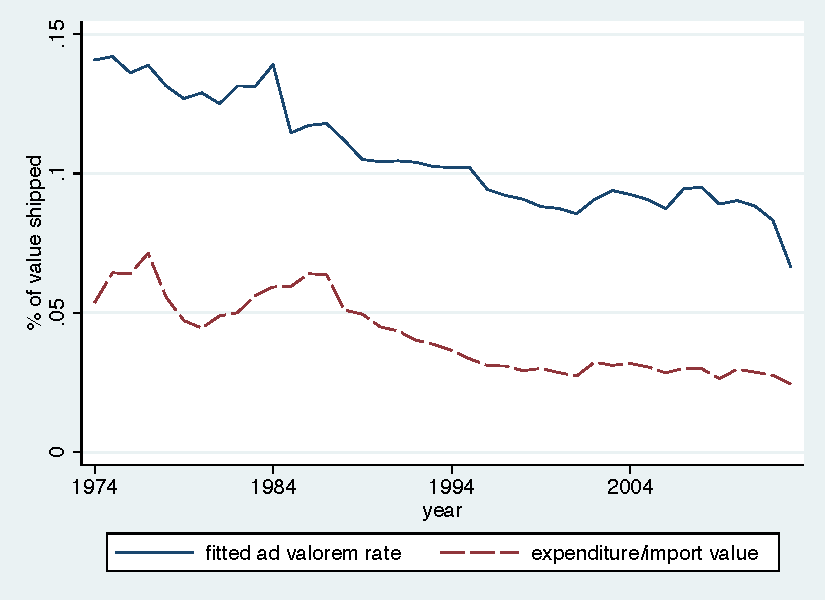
\includegraphics[width=3in, height=2.5in]{figure5_comme_hummels.pdf}
& 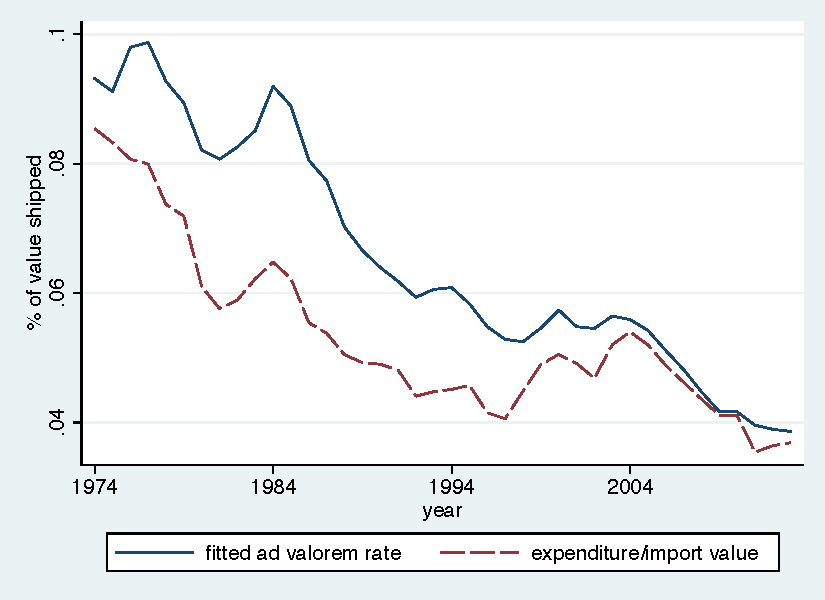
\includegraphics[width=3in,height=2.5in]{figure6_comme_hummels.pdf} \\
\end{tabular}
\end{center}
\end{figure}

\textbf{enlever figure 5 et figure 6}. 

The results stand in sharp contrast with the ones obtained with our methodology and reported in Figure \ref{fig:totalTC_compeffects_excl}. Applying Hummels' (2007) method, we obtain that the composition effects tend to mitigate the decrease in transport costs in both air and ocean shipping, in line with his results. This result is overturned when we allow for more flexibility in the role of the additive component, as depicted in Figure \ref{fig:totalTC_compeffects_excl}. Complementing the findings of Section \ref{sec:results_decomposition}, these results point out the importance of integrating the additive dimension of international transport costs, here in view of characterizing their time trends.




\subsection{At a more disaggregated level}

\textbf{A mon avis, a mettre en online appendix. Expliquer comment se fait la decomposition en secteurs primaire/manuf.}

In this Section, we characterize the time trend in international transport costs at a more disaggregated level, by distinguishing the trade flows for primary goods and manufactured goods. The evolution in transport costs over time, by transport mode (overall transport costs and composition effects excluded) are reported in \ref{fig:totalTC_compeffects_excl_manuf} for the manufacturing sector, and in Figure \ref{fig:totalTC_compeffects_excl_primary} for the primary goods.

\begin{figure}[htbp]
\caption{Transport costs (with and without composition effects), Manufacturing}
\label{fig:totalTC_compeffects_excl_manuf}
\begin{center}
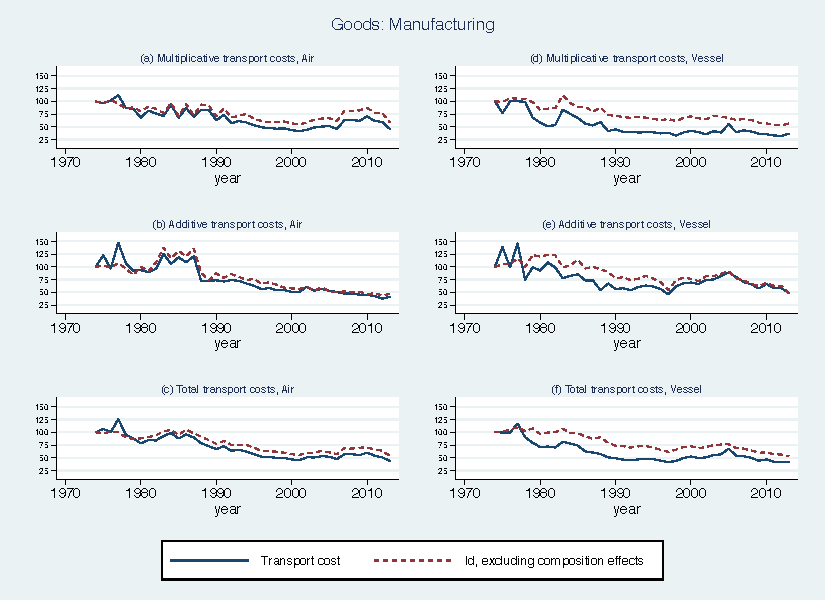
\includegraphics[height=4in]
{graph_composition_manuf.pdf}
\end{center}
\end{figure}

\begin{figure}[htbp]
\caption{Transport costs (with and without composition effects), Primary goods}
\label{fig:totalTC_compeffects_excl_primary}
\begin{center}
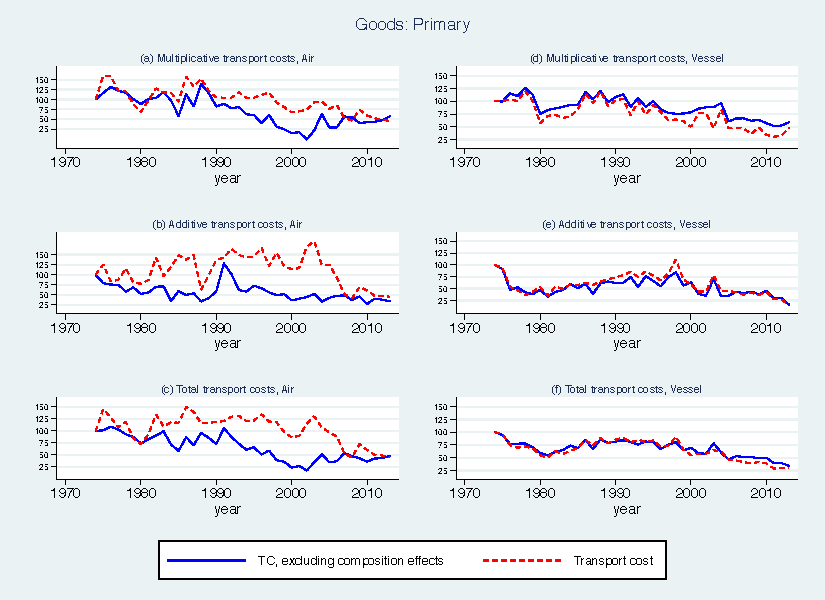
\includegraphics[height=4in]
{graph_composition_primary.pdf}
\end{center}
\end{figure}



\begin{figure}[htbp]
\caption{Share of primary goods in the value of total US imports}
\label{fig:Share_prim_goods}
\begin{center}
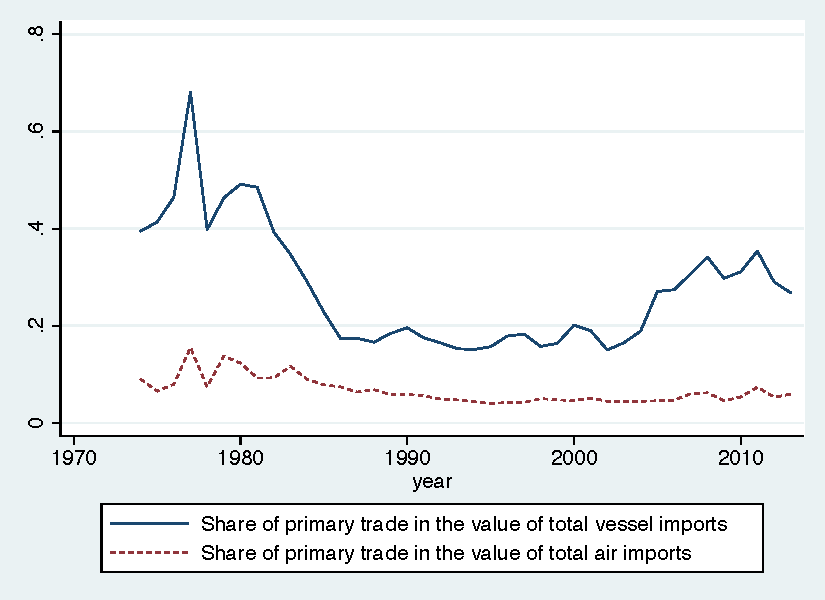
\includegraphics[height=4in]
{Share_of_primary.pdf}
\end{center}
\end{figure}

\textbf{A commenter. A mettre en Online Appendix?}

\end{document}

